\documentclass[output=paper]{LSP/langsci} 
\ChapterDOI{10.5281/zenodo.2563678}
\author{Valérie Guérin\affiliation{James Cook University}\lastand Grant Aiton\affiliation{James Cook University}}
\title{Bridging constructions in typological perspective} 
%\epigram{Change epigram in chapters/01.tex or remove it there }
\abstract{In this chapter, we undertake a cross-linguistic examination of bridging constructions, which we define as the sequence of two clauses: the first clause (called the reference clause) ends a discourse unit, the second clause (called the bridging clause) typically repeats the first clause at the beginning of a new discourse unit. Based on published language data and data from the volume, we identify three different types of constructions subsumed under the label bridging construction (\sectref{sec:guerin:2} and \sectref{sec:guerin:3}): recapitulative linkage, summary linkage, and mixed linkage. They differ in the form that the bridging clause takes on: broadly speaking, verbatim lexical recapitulation of the reference clause; a light verb summarizing the reference clause; or a mix of these two strategies. Because bridging constructions lie at the interface of discourse and syntax, we dedicate \sectref{sec:guerin:4} to explaining their discourse functions. Amid the cross-linguistic variation, we found two recurrent discourse functions: emphasizing sequentiality and cohesively structuring discourse. Finally, we establish a list of questions to guide the documentation of these linguistic patterns.}
\maketitle
%-------------------------

\begin{document}

\label{ch:1}
\section{Preliminaries}
\label{GuAi1prelim}

While reference grammars and the typological literature have a long tradition describing syntactic phenomena within a clause, cross-linguistic research beyond the level of the clause, especially the role that clause-level phenomena play in discourse structure, is comparatively scarce. This volume presents a case study of one such phenomenon, variously labelled in the literature as \textit{tail-head linkage} \citep{devries.2005}, \textit{head-tail linkage} \citep[][163]{fabian98}, \textit{tail-head recapitulation} \citep[][197]{farr99} \textit{recapitulation clauses} (\citealt[][438]{Genetti.2007}; \citealt[][17]{stirling93}), \textit{echo clauses} \citep{Heath18}, or \textit{backgrounding repetition} \citep[][10]{McKay.2008}, and the less-described variant \textit{generic verb recapitulation} \citep[][204, 337]{farr99} or \textit{summary-head linkage} \citep[][274]{Thompson.et.al.2007} to refer to constructions which contribute to discourse \isi{cohesion} and structuring in that they ``link sentences or paragraphs together, usually by \isi{repetition} of at least part of the previous clause'' \citep[][342]{Thurman1975}.\footnote{The origin of the term \textit{tail-head linkage} is unclear. Although this term has a long tradition in chemistry, its first usage in linguistics could be \citet{Longacre.1968}.}  

Tail-head linkage is found in a wide number of genetically and geographically diverse languages. It exists in \ili{Wolaitta}, an Omotic language of Ethiopia (Azeb Ahma, p.c.\ia{Ahma, Azeb}) and is attested in \ili{Bangime} (isolate, eastern Mali; \citealt{Heath18}); \ili{Biak} (Austronesian, Indonesia; \citealt{Plattel2013}); \ili{Cavineña} (Tacanan, Bolivia; \citealt{Guillaume2011}); \ili{Creek} (Muskogean, USA; \citealt{Martin1998}); \ili{Evenki} (Tungusic, Russia; \citealt{Grenoble2012}); \ili{Ngandi} (southeastern Arnhem Land, Australia; \citealt{heath1985}); \ili{Rembarrnga} (central Arnhem Land, Australia; \citealt{McKay.2008}); \ili{Tariana} (\ili{Arawak}, Brazil; \citealt{aikhenvald19}); \ili{Tirax} (\ili{Oceanic}, Vanuatu; \citealt{brotchie09}); and \ili{Yurakaré} (unclassified, Bolivia; \citealt{vangijn14}), to name a few (see also the list in \citealt[][111]{Guillaume2011}). But to the best of our knowledge, this type of linkage has never been the subject of any substantial cross-linguistic study. It is the intent of this volume to partly fill this gap, proposing in this introductory chapter general characteristics of this type of linkage and presenting in subsequent chapters descriptive studies of the phenomenon in unrelated languages.

To compare tail-head linkage across languages, we survey the relevant published literature and extract the features which define this linguistic pattern. We then formulate a comparative concept (in the sense of \citealt{haspelmath10, haspelmath16}; and \citealt{croft.2016}) presented in (\ref{GuAiex1}). As the data revealed the existence of three distinct types of linkage, we adopt the term \textsc{bridging construction} as a hypernym to avoid terminological confusion between \textit{heads} and \textit{tails}, and to capture the full range of patterns, of which only a subset may be subsumed under the labels \textit{tail-} or \textit{summary-head linkage}.\footnote{Not to be confused with the bridging implicature of \citet{clark75}. We thank Martin Haspelmath for this reference.} 

\begin{exe}
\ex	\label{GuAiex1}
\glt Bridging constructions: A comparative concept
\glt A bridging construction is a linkage of three clauses. The first clause of the construction (i.e., the reference clause) is the \isi{final clause} in a unit of discourse. The second clause (i.e., the bridging clause) recapitulates the reference clause. It usually immediately follows the reference clause but it acts as the initial (albeit non-main) clause of a new discourse unit. The primary discourse function of a bridging construction is to add structure and \isi{cohesion}: recapitulation backgrounds the proposition of the reference clause and foregrounds the clause following the bridging clause. This third clause is discourse-new and typically sequentially ordered.
\end{exe}
 
In the rest of this section, we refine the concepts in (\ref{GuAiex1}), while in the following sections we review the formal properties (\refsec{GuAi2formalcharac} and \refsec{GuAi3types}) and discourse functions (\refsec{GuAi4discourse}) of bridging constructions across individual languages. The distinction between \isi{repetition} and bridging construction is discussed in \refsec{5otherRep}. We include suggestions for future research in \refsec{GuAi6summary}. Lastly, the Appendix lists a series of questions that should be addressed when describing bridging constructions in individual languages. 

\subsection{The constructions}
\label{GuAi1.1construction}
The structure of a bridging construction is represented schematically in (\ref{GuAiex2}). There are two discourse units linked by the construction. We call the \isi{final clause} of the first unit the \textsc{reference clause} (a clause which is generally known as the \textit{tail}). The second discourse unit begins with what we label the \textsc{bridging clause} (that is, traditionally the \textit{head}), a clause which refers back to the reference clause. We adopt the convention of underlining the reference clause and bolding the bridging clause throughout this volume. 

\begin{exe}
\ex	\label{GuAiex2}
\glt [...[\underline{Reference Clause}]]\textsubscript{discourse unit} [[\textbf{Bridging Clause}]...]\textsubscript{discourse unit}
\end{exe}

The linked discourse units are typically, though not necessarily, multiclausal. The nature of these units (variously referred to in the literature as sentences or clause-chains, paragraphs or discourse episodes) remains an open question, which we address in \refsec{GuAi4discourse}. But importantly, it is the presence of both the reference and bridging clauses, their formal representation, the semantic relationship between these two clauses, and their functions in discourse that create a bridging construction and that set it apart from other clause linking techniques.

The three types of bridging constructions that we distinguish consist of a reference clause and a bridging clause. Their differences lie in the formulation of the bridging clause. The first type, called \textsc{recapitulative linkage} (formerly \textit{tail-head linkage}), involves the \isi{repetition} of the predicate of the reference clause in the bridging clause, as shown in (\ref{GuAiex3ab}). 

\begin{exe}
	\ex	\label{GuAiex3ab}
\langinfo{Nahavaq}{\ili{Oceanic}, Vanuatu}{\citealt[][259]{dimock09}}
\begin{xlist}
\ex	\label{GuAiex3a}
\gll		...en   \underline{\smash{re-tur-gcor}}     \underline{\smash{no-pon}}     \underline{\smash{no-qond}}.\\
			and   \textsc{3pl}-sew-block   \textsc{n.pref}-opening   \textsc{n.pref}-basket\\
		\glt	\sqt{...and they sewed up the opening of the basket.} \\
		\ex	\label{GuAiex3b}
\gll		\textbf{Re-tur-gcor }    \textbf{no-pon}     \textbf{no-qond},   re-gcur   i-gcisgces.\\
\textsc{3pl}-sew-block   \textsc{n.pref}-opening   \textsc{n.pref}-basket   \textsc{3pl}-cause   \textsc{3sg}-tight \\
		\glt	\sqt{After they sewed up the opening of the basket, they tightened it.} 
		\end{xlist}
\end{exe}


The second type is here called \textsc{summary linkage} (formerly \textit{summary-head linkage}). It does not repeat the predicate of the reference clause but contains in the bridging clause an \isi{anaphoric predicate}, a \isi{light verb}, a generic verb, or a \isi{demonstrative verb}, such as \textit{tangamba} `do thus' in (\ref{GuAiex4b}), which anaphorically refers to the reference clause. 



\begin{exe}
	\ex	\label{GuAiex4ab}
\langinfo{Siroi}{Papua New Guinea}{\citealt[][150]{kleef88}}
\begin{xlist}
\ex	\label{GuAiex4a}
\gll		 \underline{Piro}   \underline{\smash{mbolnge}}   \underline{\smash{ngukina}}.  \\
			garden  \textsc{loc}  planted\\
		\glt	\sqt{She planted it in the garden.} \\
		\ex	\label{GuAiex4b}
\gll \textbf{Tangamba} nu   kinyna\\
doing.thus   she   slept \\
		\glt	\sqt{After having done thus, she slept.} 
		\end{xlist}
\end{exe}


We call the third type of bridging construction \textsc{mixed linkage}. This type of construction, exemplified in (\ref{GuAiex5ab}), is a combination of recapitulative and summary linkages in that the bridging clause contains both the lexical predicate of the reference clause and a generic or demonstrative predicate.  The bridging clause in (\ref{GuAiex5b}) includes the verb \textit{reke} `cross' of the reference clause in addition to a manner demonstrative \textit{jadya} `thus' and the auxiliary \textit{ju} `be' (which are used in a type of \isi{summary linkage} in that language).

\begin{exe}
	\ex	\label{GuAiex5ab}
\langinfo{Cavineña}{Tacanan, Bolivia}{\citealt[][129]{Guillaume2011}}
\begin{xlist}
\ex	\label{GuAiex5a}
\gll		Ji-da=dya=di       \underline{ka-reke-ti-kware}  \\
good-\textsc{adj.suf}=\textsc{foc}=\textsc{emph}   \textsc{refl}-cross-\textsc{refl}-\textsc{rem.pst} \\
\glt	\sqt{I crossed well.} \\
\ex	\label{GuAiex5b}
\gll \textbf{Ka-reke-ti}      \textbf{jadya}   \textbf{ju-atsu} tapeke=piji   ara-kware\\
\textsc{refl}-cross-\textsc{refl}   thus   be-\textsc{ss}     trip.food=\textsc{dim}   eat-\textsc{rem.pst}\\
\glt	\sqt{After crossing, I ate the food.} 
\end{xlist}
\end{exe}

\subsection{The clause}
\label{GuAi1.2clause}
We take the \textsc{clause} to be a comparative concept \citep[following][672]{haspelmath10}, involving a predicate (verbal or non-verbal) and its argument(s). A \textsc{final clause} is taken to be the last clause in a series of formally linked clauses. A \isi{final clause} can be a \textsc{main clause} or a \textsc{non-main clause}. By \isi{main clause} we mean a clause that can stand by itself as an independent complete utterance. The verbal predicate of a \isi{main clause} is inflected for all required grammatical categories (i.e., it is \isi{finite}), and (generally) has a falling \isi{intonation} \citep{fitzpatrick.2000}. A \isi{main clause} can be seen as the equivalent of an independent sentence; however, we avoid the term ``sentence'' itself, as it is not readily applicable to many languages (\citealt[][132--133]{dixon10}; \citealt{Longacre1970}; \citealt{Miller1995}; \citealt{Mithun2005}). A \isi{non-main clause} cannot stand by itself as an independent complete utterance; it is dependent on another clause.\footnote{We do not consider here insubordinate clauses \citep{evans07}, which are formally non-main clauses that have gained independent status.} The dependency can be marked in any  level of the grammar, typically either (i) in the morpho-syntax: e.g., a linker marks a clause as dependent; the verbal predicate of the clause is only partially inflected or not inflected at all (i.e., it is non-\isi{finite}); or both a linker and reduced inflection occur, etc.; or (ii) in the \isi{prosody}: morpho-syntactically, the clause is inflected like a \isi{main clause} but the continuation \isi{intonation} reveals the dependency (\citealt{bolinger.1984}; \citealt[][9--10]{chafe88}; \citealt[][23--24, 31]{genetti04}; \citealt{Mithun2009}). The syntactic status of non-main clauses is notoriously difficult to define especially for some of the languages in this volume which make use of \textsc{clause chains} (i.e., non-main clauses in series). Non-main clauses have been described as adverbial clauses, pseudo-subordinate, co-subordinate, pseudo-coordinate clauses, medial clauses, or converbs. To avoid language-specific analysis of dependency types, we use the term \textsc{non-main clause} as a typologically generic cover term in this introductory chapter.\footnote{On clausal dependencies, see \citealt{cristofaro05};  \citealt{culicover.1997};  \citealt{haiman.1984}; \citealt{Haspelmath.1995}, \citealt{haspelmath2004}; \citealt[][398--417]{longacre07}; \citealt{valin84}; or  \citealt{Yuasa02}; among others.}

\subsection{Bridging constructions in discourse}
\label{GuAi1.3discours}
Some languages possess only one type of bridging construction while others have developed more. \ili{Nahavaq} seems to only use \isi{recapitulative linkage}, but in \ili{Siroi}, recapitulative and summary linkages co-exist, while \ili{Cavineña} shows all three types of linkage. Needless to say, the functions that bridging constructions can fulfil in discourse are varied. However, there are also some common trends across languages. The discursive function that is most often associated with bridging constructions is \textsc{thematic continuity} (in de Vries’ \citeyear{devries.2005} terminology). That is, the linkage is used to highlight the succession of events, as in \ili{Nahavaq} \citep[][259]{dimock09}; it supports the continuous flow of the story’s main events, such as in \ili{Siroi} \citep[][151--153]{kleef88}; and it foregrounds the ``important milestones in the story'' and ``advances the \isi{action} of the \isi{narrative}” in \ili{Cavineña} \citep[][118--120]{Guillaume2011}. This trend is possible owing to the fact that recapitulation ``transforms the repeated item from new into given information'' \citep[][224--225]{brown.2000} which adds discourse \isi{cohesion}. The concept of givenness in this context is closest to the sense of \textsc{saliency} outlined by \citet[][228]{prince81} where ``the speaker assumes that the hearer has or could appropriately have some particular thing/entity in his/her CONSCIOUSNESS at the time of hearing the utterance.'' In this sense, a bridging construction ensures that the event described in the reference clause is salient in the mind of the hearer. 

\section{Bridging constructions: formal characteristics}\label{sec:guerin:2}
\label{GuAi2formalcharac}
In \refsec{GuAi2.1layout}, we discuss the position of the reference and bridging clauses in a bridging construction, before addressing the syntactic status of these clauses in \refsec{GuAi2.2Morphosy.ref.cl} and \refsec{GuAi2.3Morphosy.brid.cl} respectively. 

\subsection{Layout}
\label{GuAi2.1layout}
A common assumption regarding the position of the clauses is that the reference clause is ``repeated in the first clause of the next chain'' \citep[][363]{devries.2005}; that is, the reference clause and the bridging clause are parts of two distinct discourse units, with the bridging clause a constituent of the second unit. This assumption holds in all languages we have seen so far. While it is typically the case that the reference clause \textit{immediately} precedes the bridging clause, it is also possible for a clause to intervene between reference and bridging clause. A case in point is the bridging clause in (\ref{GuAiex6c}) which is separated from the reference clause in (\ref{GuAiex6a}) by another clause in (\ref{GuAiex6b}). A similar phenomenon is reported in \ili{Korowai} \citepv{chapters/07Devries}.

\begin{exe}
	\ex	\label{GuAiex6ad}
\langinfo{Jingulu}{non-Pama-Nyungan, Australia} {\citealt[][]{Pensalfini}}
\begin{xlist}
\ex	\label{GuAiex6a}
\gll		Buba-ngka   \underline{dakard}     \underline{\smash{karuma-nya-yi}} \\
			fire-\textsc{all}   warm     warm-\textsc{2sg-fut}\\
		\glt	\sqt{You warm it in the fire.} \\
\ex	\label{GuAiex6b}
\gll		Nyirrma-nya-yi, \\
			make-\textsc{2sg-fut} \\
		\glt	\sqt{You’ll make it (then)} \\
\ex	\label{GuAiex6c}
\gll		\textbf{dakard}   \textbf{karuma-nya-yi},  \\
			warm    warm-\textsc{2sg-fut}\\
		\glt	\sqt{having warmed it,} \\
\ex	\label{GuAiex6d}
\gll ila-nya-yi   langa   kijurlurlu.\\
put-\textsc{2sg-fut}   \textsc{prep}   stone\\
		\glt	\sqt{you’ll put it on the stone.} 
		\end{xlist}
\end{exe}



In the corpus assembled for this volume, composed mostly of monologue narratives, a maximum of four clauses can separate the reference and the bridging clause, as in \ili{White Hmong} \citepv{chapters/05Jarkey}. 

\subsection{Morphosyntactic properties of reference clauses}
\label{GuAi2.2Morphosy.ref.cl}

The reference clause is typically cast in the declarative mood. This can arise from the discourse function of bridging constructions, linking discourse units in \isi{narrative} texts, but it may be simply a result of a data bias, as the data for this study have been drawn mainly from narratives. Occasional examples of non-declarative reference clauses include exclamative clauses in \ili{Mavea} \citepv{chapters/08Guerin}, interrogatives in \ili{Tsezic} languages \citepv{chapters/04Forker-Anker} and imperatives in \ili{Korowai}, shown in (\ref{GuAiDevex:07ab}).

\begin{exe}
\ex \label{GuAiDevex:07ab}
\langinfo{Korowai}{Papua New Guinea}{\citealt{chapters/07Devries} [this volume]}
\begin{xlist}
\ex \label{GuAiDevex:07a}						
\gll ...if-e=xa bando-xe-nè \underline{le-mén=é}\\
here-\textsc{tr=conn} bring-go-\textsc{ss} eat-\textsc{imp:2pl=ex}\\
\glt \sqt{...you should take this and eat it!}\\
\ex \label{GuAiDevex:07b}						
\gll \textbf{le-mén=daxu} noxu  lép-telo-xai=xa...\\
eat-\textsc{imp:2pl=ss} \textsc{1pl} ill-be\textsc{[non1sg]-irr=conn} \\
\glt \sqt{You must eat it and if we fall ill...} 
\end{xlist}
\end{exe}


When reference clauses are main clauses, they show no restrictions in terms of the tense, aspect, modality, negation, predicate type, etc. They can contain a verbal predicate (as in the examples cited to this point) or a nominal predicate, as shown in (\ref{GuAiAiex:08ab}). The bridging clause then repeats the nominal with a copula verb which bears a dependency marker.

\noindent\parbox{\textwidth}{\begin{exe}
\ex \label{GuAiAiex:08ab}
\langinfo{Eibela}{Papua New Guinea}{\citealt{chapters/06Aiton} [this volume]}
\begin{xlist}
\ex \label{GuAiAiex:08a}
\gll [ɛjaːgɛ	do-si=ki]\textsubscript{medial} \underline{\smash{[uʃu]}}\textsubscript{final}\\
butterfly \textsc{stat}-\textsc{med}:\textsc{pfv}=\textsc{cont} egg\\
\glt \sqt{There being a butterfly then there is an egg.}\\
\ex \label{GuAiAiex:08b}
\gll \textbf{[uʃu}	\textbf{do-si=ki]}\textsubscript{medial}	\underline{\smash{[kɛkɛbɛaːnɛ]}}\textsubscript{final}\\
egg	\textsc{stat}-\textsc{med}:\textsc{pfv}=\textsc{cont} caterpillar\\
\glt \sqt{There being an egg then there is a caterpillar.}
\end{xlist}
\end{exe}}


\subsection{Morphosyntactic properties of bridging clauses}
\label{GuAi2.3Morphosy.brid.cl}
As mentioned in \REF{GuAiex1}, bridging clauses are, at some level or other in the grammar, dependent clauses. We found three different dependency relations. First, the dependency is marked in the morphology. In some of the languages we investigated, dependent clauses show morphological modifications or morphological restrictions relative to main clauses in the tense, aspect, modality markers, etc., that they can be specified for. For example, in (\ref{GuAiDevex:07ab}) above, there is no change in mood between the reference and bridging clauses; however, the bridging clause bears a switch-reference marker, which identifies it as a dependent (and \isi{non-main clause}). In \ili{Tsezic} languages \citepv{chapters/04Forker-Anker}, bridging clauses all use converbs, which is the default strategy in these languages to express dependency (or in these languages, \isi{subordination}). In \ili{White Hmong}, bridging clauses are reduced main clauses: they cannot contain pragmatic markers usually occurring at the edge of a \isi{main clause} nor coordinators or markers of temporal sequence \citepv{chapters/05Jarkey}. 

Second, the dependency is marked in the \isi{prosody}. Some languages do not use morphological means to mark dependent clauses but utilize instead continuation \isi{prosody} to indicate the dependency. Consider \ili{Rembarrnga} \citep[][5, 10]{McKay.2008}. As in many Australian languages, a clause boundary is best defined by \isi{prosody}. All elements in a single \isi{intonation} contour are considered part of one clause. In \ili{Rembarrnga}, bridging clauses are part of the same \isi{intonation} contour as the clause that follows, indicating that they are not independent clauses. In our corpus, three languages use \isi{prosody} to indicate dependency: \ili{Mavea} \citepv{chapters/08Guerin}, \ili{Logoori} \citepv{chapters/03Sarvasy} and \ili{Jingulu} \citep{Pensalfini}. In \ili{Mavea}, both reference and bridging clauses are morphologically equivalent to main clauses. Bridging clauses are overtly marked as dependent clauses by their \isi{intonation}. The reference clause ends in a falling or level \isi{intonation}, while the bridging clause ends in a rising \isi{intonation} to indicate continuation. This is visible in Figure~\ref{GuFig3} representing the sequence in (\ref{GuAiGuex:11ac}). 

\begin{exe}
\ex \label{GuAiGuex:11ac}
\langinfo{Mavea}{\ili{Oceanic}, Vanuatu}{\citealt{chapters/08Guerin} [this volume]}
\begin{xlist}
\ex \label{GuAiGuex:11a}
\gll \underline{Ko-viris}          \underline{i-si}                 \underline{na}     \underline{kuku}. [1s]\\
\textsc{2sg}-squeeze     \textsc{3sg:irr-}go.down   \textsc{loc}    pot \\
\glt \sqt{You squeeze (out the juice) down in a pot.}\\
\ex \label{GuAiGuex:11b}
\gll \textbf{Ko-viris}          \textbf{i-si}               \textbf{na }    \textbf{kuku}   ro [1.15s] \\
\textsc{2sg}-squeeze     \textsc{3sg:irr-}go.down   \textsc{loc}    pot then\\
\glt \sqt{You squeeze (out the juice) down in a pot then,}\\
\ex \label{GuAiGuex:11c}
\gll   ko-ku-a.\\     	       
\textsc{2sg}-boil-\textsc{3sg}\\
\glt \sqt{you boil it.} 
\end{xlist}
\end{exe}

\begin{figure}[ht]
% \fbox{
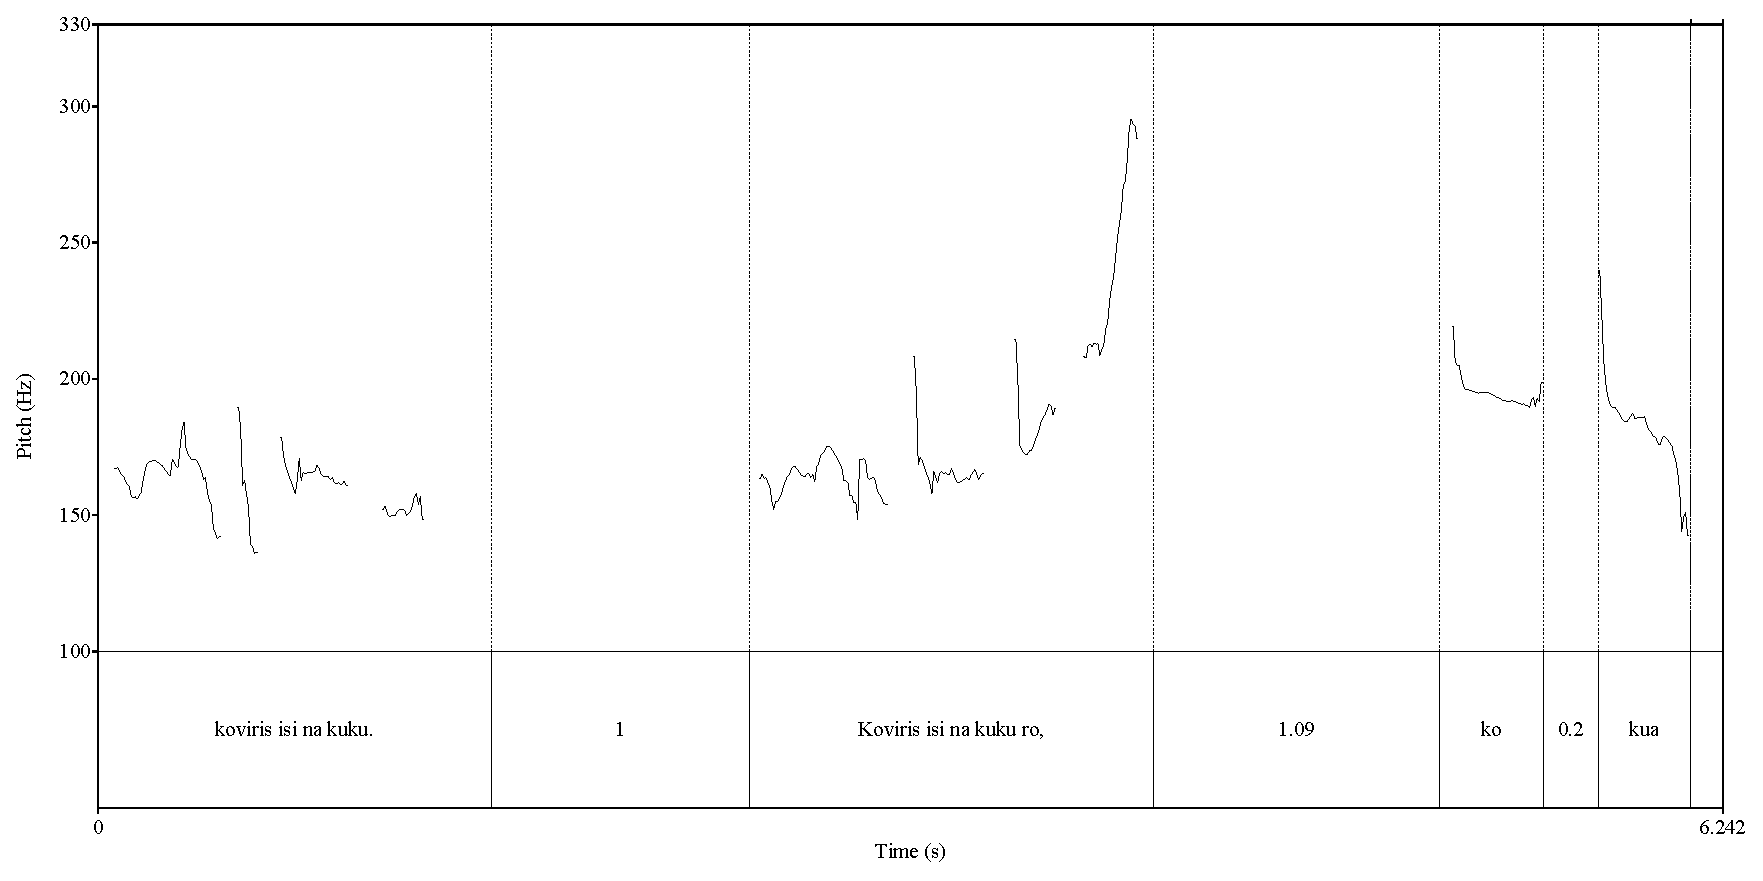
\includegraphics[width=4.8in]{figures/guerinFig3x.eps}
\caption{Intonation contour of example (\ref{GuAiGuex:11ac}) extracted with PRAAT. \label{GuFig3}}
\end{figure}


In \ili{Mavea}, dependent clauses need not be marked morphologically. Adverbials also seldom make use of overt \isi{non-main clause} markers (e.g., complementizer or subordinator). They resort instead to \isi{prosody} (e.g., rising \isi{intonation}) to mark continuation and indicate grammatical or discourse dependency. The \ili{Jingulu} data concur: the bridging clause is marked with the same \isi{intonation} that encodes given information. However, in the absence of fluent speakers today, the \ili{Jingulu} data is less conclusive (Rob \citeauthor{Pensalfini}, p.c.).\nocite{PRAAT}

\ili{Logoori} is interesting in that respect. In this language (as in other \ili{Bantu} languages), the predicate of the first clause in the chain is \isi{finite}, the medial and final clauses of the chain are non-\isi{finite}. Thus, in \ili{Bantu} bridging constructions, the reference clause is non-\isi{finite} (being the last in the chain) and the bridging clause is \isi{finite} (being the first in the chain). However, bridging clauses in \ili{Logoori} are also prosodically dependent, while reference clauses are prosodically main clauses (see \citealt{chapters/03Sarvasy} [this volume]).

Third, the dependency is marked both in the morphology and the \isi{prosody}. Some languages may use both morphology and non-final \isi{intonation} to mark clause dependency. In the Australian language \ili{Ngandi}, the bridging clause contains a morpheme indicating \isi{subordination}. In addition, the clause ends on a rising continuation pitch while the clause following it has falling terminal pitch \citep[99]{heath1985}. 

As these different dependency strategies reveal, the general profile of a language influences the formal characteristics of the bridging constructions in that language (see  \citealt{devries.2005}; \citealt[][898]{seifart10}). It is worth mentioning too that in some cases, a subordinator is present to overtly mark the bridging clause as dependent. Thus in \ili{White Hmong}, the temporal relationship between the reference and the bridging clause can be explicit, as in (\ref{GuAiJaex:09ab}) with \textit{thaum} `when' or implied, as in (\ref{GuAiJaex:10ab}). 


\begin{exe}
\ex \label{GuAiJaex:09ab}
\langinfo{White Hmong}{Hmong-Mien, Laos}{\citealt{chapters/05Jarkey} [this volume]}
\begin{xlist}
\ex \label{GuAiJaex:09a}
\gll ...ces \underline{\smash{nws}} \underline{\smash{poj.niam}} \underline{\smash{thiaj}} \underline{xauv.xeeb} \underline{tau} \underline{ob} \underline{\smash{leeg}} \underline{tub} \underline{ntxaib}.\\
and.then \textsc{3sg} woman so.then give.birth get two \textsc{clf} son twin\\
\glt \sqt{...and so then his wife gave birth to twin boys.}\\
\ex \label{GuAiJaex:09b}
\gll \textbf{Thaum} \textbf{xauv.xeeb} \textbf{tau} \textbf{nkawd}...\\     	      
    when  give.birth get \textsc{3du}\\
\glt \sqt{When she had given birth to them...} 
\end{xlist}
\end{exe}

\begin{exe}
\ex \label{GuAiJaex:10ab}
\begin{xlist}
\ex \label{GuAiJaex:10a}
\gll \textsc{ces} \underline{txawm} \underline{mus} \underline{ntsib} \underline{\smash{nraug}} \underline{\smash{zaj}}.\\
and.then then go meet young dragon\\ 
\glt \sqt{and then (she) went (and) met a young dragon.}\\
\ex \label{GuAiJaex:10b}
\gll \textbf{Ntsib} \textbf{nraug} \textbf{zaj},\\		
 meet young dragon \\ 
\glt \sqt{(She) met the young dragon...}
\end{xlist}
\end{exe}

In this volume, we do not separate out bridging clauses with an overt lexical subordinator such as (\ref{GuAiJaex:09ab}) from bridging clauses whose sole indicators of dependency are \isi{prosodic} like (\ref{GuAiJaex:10ab}) or morphological. Although there could be discourse differences between the different dependency markings, we do not have enough data at this stage to argue that (\ref{GuAiJaex:09ab}) is a less prototypical bridging construction than (\ref{GuAiJaex:10ab}) for example.

\section{Types of bridging constructions}\label{sec:guerin:3}
\label{GuAi3types}
The two types of bridging constructions most commonly described across languages are \textsc{recapitulative linkage} and \textsc{summary linkage}. They can be distinguished on the basis of the predicate that their bridging clause contains: in \isi{recapitulative linkage}, the bridging clause repeats at least the predicate of the reference clause either verbatim or with a close paraphrase; whereas the bridging clause of a \isi{summary linkage} contains an \isi{anaphoric predicate} recapping the event/state of the reference clause. A third type of bridging construction emerged from our data collection and comparative studies. We call it here \textsc{mixed linkage}. This type of bridging construction combines both recapitulative and summary linkages. We discuss these three types of linkage in turn below.

\subsection{Recapitulative linkage}
\label{GuAi3.1recap}
Every definition of bridging construction that we encountered in the literature refers to a portion of discourse being \textit{repeated} elsewhere. What is generally assumed is that the \isi{repetition} is more or less exact, i.e., exact enough so that the reference and bridging clauses can be identified as expressing the same proposition with the same lexical items. There exist, however, many different types of \isi{repetition} \citep[][224]{brown.2000}. We take as our starting point a bridging clause with apparent verbatim \isi{repetition}. In \ili{Tirax} (as in many other \ili{Oceanic} languages of Vanuatu), the bridging clause in (\ref{GuAiex:12b}) is morphologically identical to the reference clause in (\ref{GuAiex:12a}). The only difference is the rising \isi{intonation} which marks the bridging clause as non-final, as described for (\ref{GuAiGuex:11ac}).


\begin{exe}
\ex \label{GuAiex:12ac}
\langinfo{Tirax}{\ili{Oceanic}, Vanuatu}{\citealt[][309]{brotchie09}}
\begin{xlist}
\ex \label{GuAiex:12a}
\gll \underline{tnah}   \underline{haxal}   \underline{i=mɛ}\\
devil   \textsc{indf}   \textsc{3sg:real}=come \\
\glt \sqt{and a devil came along.} (falling \isi{intonation})\\
\ex \label{GuAiex:12b}
\gll \textbf{tnah}  \textbf{ haxal}   \textbf{i=mɛ} \\
devil   \textsc{indf}   \textsc{3sg:real}=come\\
\glt \sqt{A devil came,} (rising \isi{intonation})\\
\ex \label{GuAiex:12c}
\gll   i=rŋo...\\     	       
\textsc{3sg:real}=hear\\
\glt \sqt{and he heard...} 
\end{xlist}
\end{exe}



The term \textsc{verbatim} \isi{repetition}, then, does not precisely represent the content of a bridging clause (despite this common assumption regarding \isi{recapitulative linkage}): at the very least, changes required to accord a bridging clause dependent status are generally applied, be they purely intonational as in (\ref{GuAiGuex:11ac}), or morphological as in (\ref{GuAiex:13ab}), where the predicate `become strong' is marked as non-final in (\ref{GuAiex:13b}).


\begin{exe}
\ex \label{GuAiex:13ab}
\langinfo{Nabak}{Papua New Guinea}{\citealt[][164]{fabian98}}
\begin{xlist}
\ex \label{GuAiex:13a}
\gll ...met-me     \underline{ku-mann}     \underline{\smash{ma-katik-ngang}}  \underline{be-in}\\
go-\textsc{med:3sg:ds}   nail-\textsc{med:1pl:ds}   \textsc{cont}-strong-\textsc{nmlz}   become-\textsc{3sg:prs}\\
\glt \sqt{...and it goes [in its proper place] and we nail it and [the floor] becomes strong.} \\
\ex \label{GuAiex:13b}
\gll \textbf{Ku-mann}     \textbf{katik-ngang}    \textbf{be-me}... \\
nail-\textsc{med:1pl:ds}   strong-\textsc{nmlz}     become-\textsc{med:3sg:ds}\\
\glt \sqt{We nail it and it becomes strong...} 
\end{xlist}
\end{exe}

\noindent
The \ili{Nabak} example also demonstrates that although typically a single reference clause is repeated in the bridging clause, it is possible to find two clauses repeated in their entirety. The clauses with predicates `nail' and `become strong' are both repeated in the bridging clause in (\ref{GuAiex:13b}). We have not yet found more than two clauses repeated.

Departure from verbatim \isi{repetition} affects different constituents of the reference clause. Adverbials or arguments may be omitted or the verbal inflection may differ. At least implicitly, the predicate of the reference and bridging clauses is expected to remain identical, but as we show below, the predicate is not immune to replacement. In the following sections we review four types of variation found in the languages surveyed: (1) modifications, the bridging and reference clause contain the same information but in different order or form; (2) \isi{omission}, the bridging clause omits some material present in the reference clause; (3) \isi{addition}, the bridging clause contains information, whether lexical or grammatical, which was not present in the reference clause; (4) \isi{substitution}, where some of the information in the reference clause is replaced in the bridging clause; and (5) a mixture of these features. What is common to all cases of variation (and crucial for bridging constructions) is that the propositional content of the bridging clause is equivalent to the content in the reference clause, with no additional information added to the bridging clause.

\subsubsection{Modifications}
\label{GuAi311modif}
Modification refers to cases where bridging clauses do not contain omissions from the reference clause nor additions per se, but are not strictly verbatim either. Modification may affect the lexical content of the bridging clause. For example, full \isi{NPs} in a reference clause may be pronominalized in the bridging clause, as in the \ili{Oceanic} language \ili{Lolovoli}. The object in the reference clause (\textit{diringigi} `the stone oven') in (\ref{GuAiex:14a}), is repeated in pronominal form (=\textit{e} `\textsc{3sg.o}') in the bridging clause (\ref{GuAiex:14b}). Similar facts apply to \ili{Cavineña}: the object \textit{tapeke} `food' in (\ref{GuAiex:15a}) is pronominalized with the demonstrative \textit{tumeke} `that' in (\ref{GuAiex:15b}). Nothing in the grammar of these languages would prevent a full NP from occurring in a \isi{dependent clause}.


\begin{exe}
\ex \label{GuAiex:14ac}
\langinfo{Lolovoli}{\ili{Oceanic}, Vanuatu}{\citealt[][427]{hyslop01}}
\begin{xlist}
\ex \label{GuAiex:14a}
\gll \underline{Da=mo}     \underline{sio}     \underline{na}   \underline{\smash{diringi-gi}}\\
\textsc{1pl:incl=real}    lay.stones   \textsc{acc}   stone.oven-\textsc{assoc}\\
\glt \sqt{We lay stones for the stone oven.} \\
\ex \label{GuAiex:14b}
\gll \textbf{Da=mo}    \textbf{sio=e}  mo   rovo,  \\
\textsc{1pl:incl=real}   lay.stones=\textsc{3sg:o}   \textsc{real}   finish  \\
\glt \sqt{We lay all the stones,}\\
\ex \label{GuAiex:14c}
\gll ale   da=mo     goa    na   qeta-gi... \\
\textsc{conj}   \textsc{1pl:incl=real}    scrape.dirt  \textsc{acc}   taro-\textsc{assoc}\\
\glt \sqt{then we scrape the dirt off the taro...}
\end{xlist}
\end{exe}


\begin{exe}
\ex \label{GuAiex:15ab}
\langinfo{Cavineña}{Tacanan, Bolivia}{\citealt[][129]{Guillaume2011}}
\begin{xlist}
\ex \label{GuAiex:15a}
\gll Ka-reke-ti      jadya   ju-atsu   \underline{\smash{tapeke=piji}}   \underline{ara-kware}\\
\textsc{refl}-cross-\textsc{refl}   thus   be-\textsc{ss}     trip.food=\textsc{dim}   eat-\textsc{rem.pst}\\
\glt \sqt{After crossing, I ate the food.}\\
\ex \label{GuAiex:15b}
\gll \textbf{Tumeke} \textbf{ara-tsu} era     ijeti   peta-ya. \\
that     eat-\textsc{ss}     \textsc{1sg:erg}   sun   look.at-\textsc{ipfv}  \\
\glt \sqt{After eating that (food), I looked at the sun (to know what time it was).}
\end{xlist}
\end{exe}


Other modifications include word order: the order of the phrases in the reference and bridging clauses does not match. For example in \ili{Sunwar}, \textit{aga} is emphasized and placed at the end of the refence clause in (\ref{GuAiex:16a}), whereas in the bridging clause in (\ref{GuAiex:16b}), it is restored to its non-emphasized position.


\begin{exe}
\ex \label{GuAiex:16ab}
\langinfo{Sunwar}{Himalayan, Nepal}{\citealt[][391]{schulze73}}
\begin{xlist}
\ex \label{GuAiex:16a}
\gll Minu   meko  \underline{\smash{khuy}}     \underline{oo-ma}     \underline{‘baakt}   \underline{\smash{aga}}\\
and   these   thieves   enter-\textsc{3pl}   ?  inside\\
\glt \sqt{And the thieves entered into the house.} \\
\ex \label{GuAiex:16b}
\gll \textbf{khuy}     \textbf{aga}     \textbf{oo-ma }    \textbf{‘baakta} \\
thieves   inside     enter-\textsc{3pl}   ? \\
\glt \sqt{The thieves having entered...}
\end{xlist}
\end{exe}

\noindent
Placement at the end of a clause for emphasis is not a feature associated with a particular \isi{clause type} in Sunwar. Although more common in reference clauses, it is also found in bridging clauses \citep[][391]{schulze73}. 

\subsubsection{Omissions}
\label{GuAi312omiss}
Omissions in the bridging clause target lexical items, in particular arguments and adverbials. This is the case in \ili{Ono} \citep[][121]{Phinnemore1998} and \ili{Wambon} \citep{devries.2005}. In \ili{Wambon} in (\ref{GuAiex:17b}), it is the adverbial \textit{alipke} ‘afternoon’ that is not included in the bridging clause.

\begin{exe}
\ex \label{GuAiex:17ab}
\langinfo{Wambon}{Papua New Guinea}{\citealt[][373]{devries.2005}}
\begin{xlist}
\ex \label{GuAiex:17a}
\gll Sanopkuniv-eve   ilo     nggapmo-kndevan-o   ko \underline{\smash{alipke-lo}}   \underline{ndave-levambo}\\
Tuesday-that    go.down:\textsc{ss}   cut-\textsc{1pl:prs-conn}  go:\textsc{ss} afternoon-\textsc{ss}  return-\textsc{1pl:pst}\\
\glt \sqt{On Tuesday afternoon we went down and cut (trees) until we returned in the late afternoon.}\\
\ex \label{GuAiex:17b}
\gll \textbf{ndano} la-levambon-o... \\
return:\textsc{ss}   sleep-\textsc{1pl:pst-conn} \\
\glt \sqt{Having returned, we slept and...}
\end{xlist}
\end{exe}

Ellipsis in the bridging clause can also affect grammatical morphemes. In \ili{Sunwar}, the evidential marker can be omitted from a bridging clause \citep[][392]{schulze73}. Whether it must be omitted in any \isi{non-main clause} is unclear at this stage. In \ili{Paluai} in (\ref{GuAiex:18b}), the bridging clause does not repeat the aspect marker of the reference clause (namely \textit{pe} ‘perfective’), although there are no restrictions on aspectual marking in non-main clauses in \ili{Paluai} \citep[][419]{Schokkin13}.

\noindent\parbox{\textwidth}{%
\begin{exe}
\ex \label{GuAiex:18ac}
\langinfo{Paluai}{\ili{Oceanic}, Admiralties}{\citealt[][116]{Schokkin14}}
\begin{xlist}
\ex \label{GuAiex:18a}
\gll \underline{\smash{Wurê-pe}}   \underline{suwen }    \underline{suk}\\
\textsc{1pl:excl-pfv}  move.down  shore\\
\glt \sqt{We went down to the shore.} \\
\ex \label{GuAiex:18b}
\gll \textbf{Wurê-suwen}      \textbf{suk}  \textbf{ a} \\
\textsc{1pl:excl-}move.down    shore  and    \\
\glt \sqt{we went down to the shore and}\\
\ex \label{GuAiex:18c}
\gll wurê-pe   pit   nêm     la   kel \\
\textsc{1pl:excl-pfv} jump   be.finished   go.to   canoe\\
\glt \sqt{we boarded a canoe.}
\end{xlist}
\end{exe}}



Determining what portion of the reference clause can be repeated or omitted and whether there are functional differences between exact and non-exact repetitions remain open questions. It could be that the choice of verbatim versus partial \isi{repetition} is constrained by language specific features. In \ili{Yurakaré}, for example, the verb’s arguments are rarely repeated in the bridging clause. This is a general tendency in the language, and not a specific feature of bridging constructions: topical arguments are not repeated \citep[][295--296]{vangijn14}. 

\subsubsection{Additions}
\label{GuAi313add}
Additions are instances where information present in the bridging clause is not present in the reference clause. So far, additions we have found are aspectual or lexical (added \isi{NPs}). An example of lexical \isi{addition} is given in \ili{Ma Manda} in (\ref{GuAiex:19ab}). The subject argument in the reference clause is expressed in the form of agreement (\textsc{1pl}) on the verb, but in the bridging clause, a full NP is introduced, referring to a different person–number value, namely \textsc{3pl}.


\begin{exe}
\ex \label{GuAiex:19ab}
\langinfo{Ma Manda}{Papua New Guinea}{\citealt{Pennington2015}}
\begin{xlist}
\ex \label{GuAiex:19a}
\gll \underline{blaakam}   \underline{\smash{ta-waam-ang}}\\
weed     do-\textsc{prs:1pl-hab}\\
\glt \sqt{we do the weeding.} \\
\ex \label{GuAiex:19b}
\gll  \textbf{taam-taam=pû}   \textbf{blaakam}   \textbf{ta-maa-kong-ka}\\
female-\textsc{pl=nom}   weed     do-\textsc{compl}{}-throw-\textsc{ss}\\
\glt \sqt{The women doing all the weeding, and...}
\end{xlist}
\end{exe}


An example of aspectual \isi{addition} in the verb phrase is given in (\ref{GuAiGuex:20ac}). The predicate in (\ref{GuAiGuex:20b}) is modified in (\ref{GuAiGuex:20c}) by the predicate -\textit{v} `say' which acts, in this construction, as a phasal predicate \citep[][342]{guerin11}.


 \begin{exe}
 \ex \label{GuAiGuex:20ac}
 \langinfo{Mavea}{\ili{Oceanic}, Vanautu}{\citealt{chapters/08Guerin} [this volume]}
\begin{xlist}
\ex \label{GuAiGuex:20a}
\gll    i-oele, ko-arvulesi i-lo-\H{v}a \\     	       
  \textsc{3sg:irr}-oil \textsc{2sg}-stir  \textsc{3sg:irr-ipfv}-go\\
\glt \sqt{it [is becoming] oil, you keep stirring} 
\ex \label{GuAiGuex:20b}
\gll   ko-rong     \underline{sama-na}               \underline{mo-rororo}.             \\     	       
 \textsc{2sg}-hear  froth-\textsc{3sg:poss}     \textsc{3sg}-\textsc{ideo}.noise \\
\glt \sqt{[until] you hear its froth sizzling.} 
\ex \label{GuAiGuex:20c}
\gll     \textbf{sama-na}  \textbf{ mo-v }           \textbf{i-rororo}     mal  mo-noa         ne     \\     	       
 froth-\textsc{3sg:poss}  \textsc{3sg}-say   \textsc{3sg}-\textsc{ideo}.noise \textsc{dem}  \textsc{3sg}-cooked   \textsc{foc}  \\
\glt \sqt{[when] its froth starts to sizzle, \textsc{it} is cooked.} 
\end{xlist}
\end{exe}

Additions may clarify or refine information that is implicit in the reference clause, for instance by expressing an argument as a lexical noun phrase rather than as an agreement marker, or may offer a different aspectual perspective, but additions still express the same fundamental proposition found in the reference clause.

\subsubsection{Substitution}
\label{GuAi314subst}
Substitutions are replacements targeting elements in the verb phrase of the reference clause. First, we found instances of the \isi{substitution} of only grammatical information. Consider the \ili{Ma Manda} example in \REF{GuAiex:19ab} above. The verbs are lexically identical in both clauses, but the reference clause is cast in the habitual aspect, whereas the bridging clause marks completion. Although habitual aspect is restricted to main clauses in \ili{Ma Manda}, completive can be found in both clause types. Another case may be seen in \ili{Tsezic} languages \citepv{chapters/04Forker-Anker}: the \isi{finite} or tensed verb form in the reference clause is replaced with a \isi{converb} form. Finally, in \ili{White Hmong} \citepv{chapters/05Jarkey} aspect systematically shifts between the reference clause and the bridging clause for rhetorical effect.

Second, \isi{substitution} may target the lexical verb. Lexical \isi{substitution} involves cases where the bridging verb is a synonym of the reference verb. This is shown in (\ref{GuAiex:21ab}), where two different verbs `tie with a knot' and `bind' are used in the reference and bridging clauses respectively. 

\begin{exe}
\ex \label{GuAiex:21ab}
\langinfo{Nabak}{Papua New Guinea}{\citealt[][164]{fabian98}}
\begin{xlist}
\ex \label{GuAiex:21a}
\gll mam-be-mti     \underline{\smash{za-nup}}\\
\textsc{cont}-put-\textsc{med:ss}   tie.with.a.knot-\textsc{1pl:prs} \\
\glt \sqt{[we] put it [in place on the house] and tie it [down].} \\
\ex \label{GuAiex:21b}
\gll  \textbf{Eli-mann}...\\
bind-\textsc{med:1pl:ds}\\
\glt \sqt{After we bind it...}
\end{xlist}
\end{exe}



Similar facts are reported in \ili{Matsigenka}-\ili{Spanish} \citepv{chapters/02Emlen}, \ili{Ma Manda} \citep{Pennington2015} and \ili{Eibela} in (\ref{GuAiAiex:22ab}), where both verbs `shave thin' and `make flat' refer to the same event and describe two facets of the same procedure. 


\begin{exe}
\ex \label{GuAiAiex:22ab}
\langinfo{Eibela}{Papua New Guinea}{\citealt{chapters/06Aiton} [this volume]}
\begin{xlist}
\ex \label{GuAiAiex:22a}
\gll \underline{[sɛːli}	\underline{gaːlɛ-mɛi]}\textsubscript{final}\\
properly	shave.thin-\textsc{hypoth}\\
\glt \sqt{(You) should shave it properly}\\
\ex \label{GuAiAiex:22b}
\gll \textbf{[sɛli}	\textbf{ɛmɛlɛ-si]}\textsubscript{medial}\\
properly	make.flat-\textsc{med}:\textsc{pfv}\\
\glt \sqt{Flatten it properly (by shaving)..}
\end{xlist}
\end{exe}




Although hyponymy and (partial) synonymy are not always easily distinguishable from one another, in a few languages, we find cases of hyponymy. The bridging clause contains a verb whose semantics is more general than that of the verb of the reference clause. This is reported in \ili{Siroi} \citep[][151]{kleef88} and in \ili{Ono}, shown in (\ref{GuAiex:23ab}). The verb `take' in the bridging clause in (\ref{GuAiex:23b}) is a hypernym which refers to the more specific hyponym `grab' in the reference clause in (\ref{GuAiex:23a}).

\begin{exe}
\ex \label{GuAiex:23ab}
\langinfo{Ono}{Papua New Guinea}{\citealt[][122]{Phinnemore1998}}
\begin{xlist}
\ex \label{GuAiex:23a}
\gll eŋe  kiŋzaŋ.kaŋzaŋ  wie     ŋerep   \underline{mararak-ko-i}\\
they  suddenly  get.up:\textsc{ss}   girl   grab-\textsc{3pl}-?\\
\glt \sqt{They suddenly grabbed the girl.} \\
\ex \label{GuAiex:23b}
\gll  \textbf{ma-u}    \textbf{paki}\\
take-\textsc{3pl:ds}   after:\textsc{ds} \\
\glt \sqt{After they took (her)...}
\end{xlist}
\end{exe}


On the other hand, in \ili{White Hmong} \citepv{chapters/05Jarkey} and in \ili{Timbe}, reported in (\ref{GuAiex:24ab}), the verb of the bridging clause is more specific in meaning than the verb of the reference clause (here, \textit{climb} > \textit{get to}). In Foster’s (\citeyear{foster81}) words, (\ref{GuAiex:24ab}) acts ``as if it is a correction or a refinement of the final verb'' of the previous clause.

\noindent\parbox{\textwidth}{%
\begin{exe}
\ex \label{GuAiex:24ab}
\langinfo{Timbe}{Papua New Guinea}{\citealt[][42]{foster81}}
\begin{xlist}
\ex \label{GuAiex:24a}
\gll hikakmâ   emelâk \underline{Bondâ} \underline{\smash{meyeat}}. \\
carrying   already Bondâ they.got.to\\
\glt \sqt{and carrying (her child) they made it to Bondâ.} \\
\ex \label{GuAiex:24b}
\gll  \textbf{Bondâ } \textbf{gayeat}     âmâ   ga...\\
 Bondâ they.climbing.to   when   climbing \\
\glt \sqt{When they had climbed to Bondâ they climbed to...}
\end{xlist}
\end{exe}}


Constructions with non-matching verbs in the reference and bridging clauses raise challenging questions about the limits of bridging constructions: if the predicates in the reference and bridging clause are not identical but are synonyms, should we still consider the constructions involving \isi{substitution} as bridging constructions, albeit ``atypical''? What if the predicates are not synonyms but show different facets or perspectives of the same event? Consider example (\ref{GuAi25ab}) from \ili{Tsez}:

\begin{exe}
	\ex	\label{GuAi25ab}
\langinfo{Tsez}{Nakh-Daghestanian}{\citealt{chapters/04Forker-Anker} [this volume]}
	\begin{xlist}
		\ex	\label{GuAi25a}
		\gll	...\underline{kid}  	\underline{xan-dä\smash{ɣ}or}   		\underline{\smash{y}-ik’i-n}\\
			 girl(\textsc{ii}) 	khan-\textsc{apud.vers} 	\textsc{ii}-go-\textsc{pst.uw} \\
		\glt	\sqt{...the girl went to the king.}

		\ex	\label{GuAi25b}
		\gll			\textbf{elo-r}    	\textbf{y-ay-nosi}... \\
			there-\textsc{lat}	\textsc{ii}-come-\textsc{ant.cvb} 	  \\
		\glt	\sqt{After she arrived there,...}
	\end{xlist}
\end{exe}

\noindent
In this example, a verb of movement in the reference clause is replaced by another in the bridging clause (go > come) resulting in a different deictic orientation. Should these instances be considered less like bridging constructions and more like \textsc{paraphrases} defined by \citet[][382--383]{longacre07} as inexact \isi{repetition} with a gain or loss of information? The boundary here is fuzzy, and it is not immediately obvious whether there is a clear and categorical distinction between bridging constructions with separate predicates and paraphrases. The answer, we believe, lies in the function of these types of constructions: by looking at both formal and functional features, we assume it is possible to distinguish bridging constructions from paraphrases and other forms of \isi{repetition}. This rationale, however, requires further research (see also \sectref{sec:guerin:5}).

\subsection{Summary linkage}
\label{GuAi32summ.link}
At the extreme end of the \isi{substitution} spectrum, we reach cases where the lexical verb of the reference clause, its argument, and accompanying adjuncts are replaced with a generic \isi{light verb} that has no lexical relation to the verb of the reference clause. The relation between the reference and the bridging clause is nevertheless maintained because the verb of the bridging clause is understood to summarize or anaphorically refer to the preceding discourse unit.

Across languages, two major types of verbs are used to form the bridging clause of a \isi{summary linkage}. First, a verb with generic meaning is used, such as \textit{nu} in (\ref{GuAiex:26b}).

\begin{exe}
\ex \label{GuAiex:26ab}
\langinfo{Jingulu}{non-Pama-Nyungan, Australia} {\citealt{Pensalfini}}
\begin{xlist}
\ex \label{GuAiex:26a}
\gll \underline{Marlarluka-rni}    \underline{\smash{ganya-marri}}  \underline{\smash{jad.bili}}. \\
old.man-\textsc{erg}     sing-\textsc{rem.pst}    block\\
\glt \sqt{Old people sang them to block them.} \\
\ex \label{GuAiex:26b}
\gll  \textbf{Marlarluka}   \textbf{wurru-nu},...\\
 old.man   \textsc{3pl}-\textsc{aux:pst}\\
\glt \sqt{The old people did that,...} 
\end{xlist}
\end{exe}

This generic or \isi{light verb} is often accompanied by a deictic element, as in \ili{Yurakaré} \citep[][295]{vangijn14} and \ili{Tariana} with the manner deictic \textit{kay} `thus' in (\ref{GuAiex:27c}) (see also the paragraph markers of \citealt[][701]{Loos1963}).

\begin{exe}
\ex \label{GuAiex:27ad}
\langinfo{Tariana}{\ili{Arawak}, northwest Amazonia}{\citealt[][578]{aikhenvald2003}}
\begin{xlist}
\ex \label{GuAiex:27a}
\glt \sqt{I went early, there I fished for aracú fish and went round,}\\ \vspace{-0.2in}
\ex \label{GuAiex:27b}
\gll  \underline{\smash{lape-pe-se}}     \underline{nu-emhani-na}\\
 muddy.lake-\textsc{pl-loc}  \textsc{1sg}-walk-\textsc{rem.pst:vis}\\
\glt \sqt{I went round in a muddy lake.}\\
\ex \label{GuAiex:27c}
\gll  \textbf{kay}   \textbf{nu-ni}\\
 thus   \textsc{1sg}-do\\
\glt \sqt{Having done this,}\\
\ex \label{GuAiex:27d}
\gll  dekina     nu-dia     nu-mara   nu-nu-na-pita\\
 afternoon   \textsc{1sg}-return   \textsc{1sg}-drift   \textsc{1sg}-come-\textsc{rem.pst:vis-again}\\
\glt \sqt{I drifted downstream again in the afternoon}
\end{xlist}
\end{exe}



The second strategy to form a \isi{summary linkage} is to use a \isi{pro-verb}, as in \ili{Aguaruna} in (\ref{GuAiex:28b}), or a \isi{demonstrative verb} expressing manner \citep[see][]{guerin15}, such as \textit{kwamun} `do like that' in (\ref{GuAiex:29b}). In these cases, the verb itself has deictic or anaphoric reference as part of its meaning.

\begin{exe}
\ex \label{GuAiex:28ac}
\langinfo{Aguaruna}{Jivaroan, Peru}{\citealt[][500]{overall17}}
\begin{xlist}
\ex \label{GuAiex:28a}
\gll \underline{mi=na}    \underline{\smash{apa-hu}}     \underline{\smash{maŋkahatu-a-u}}    \underline{\smash{a-yi}}\\
 \textsc{1sg=acc}   father-\textsc{poss:1sg}   kill:\textsc{1pl:obj-pfv-nmlz}  \textsc{cop-rem.pst:3:decl}\\
\glt \sqt{my father killed a person} \\
\ex \label{GuAiex:28b}
\gll  \textbf{nu-ni-ka-mata\~\i}\\
 \textsc{ana-vblz:intr-pfv:seq-1/3:ds}\\
\glt \sqt{(he) having done that’ or `and because of that}\\
\ex \label{GuAiex:28c}
\gll auhu-tsu-u=ka     papi=na=ka     puhu-ya-ha-i\\
 study\textsc{-neg-nmlz=top}   book=\textsc{acc=top}   live-\textsc{rem.pst-1sg-decl}\\
\glt \sqt{I was unable to study}
\end{xlist}
\end{exe}


\begin{exe}
\ex \label{GuAiex:29ab}
\langinfo{Yongkom}{Papua New Guinea}{\citealt[][66]{christensen13}}
\begin{xlist}
\ex \label{GuAiex:29a}
\gll \underline{Anon}    \underline{ok}   \underline{an-imam-ɛɛn}.\\
 dog   water   eat-\textsc{hab-3:m}\\
\glt \sqt{The dog was drinking water.}\\ 
\ex \label{GuAiex:29b}
\gll \textbf{Kwamun-ɛ} yikabom   bikn-ɛ...\\
do.like-\textsc{sm}   lizard    hid-\textsc{sm}\\
\glt \sqt{He did that [and then] the lizard hid...}
\end{xlist}
\end{exe}


\ili{Eibela} uses a third possibility: the durative auxiliary \textit{hɛnaː} which forms a bridging clause, as shown in (\ref{GuAiAiex:30c}).

\begin{exe}
\ex \label{GuAiAiex:30ac}
\begin{xlist}
\ex \label{GuAiAiex:30a}
\gll	[ɛimɛ	oɡa	ɛ	ɡɛ-mɛna=ta]\textsubscript{medial}	\underline{\smash{[holo}}	\underline{\smash{anɛ-obo]}}\textsubscript{final}\\
already	pandanus	seedling	plant-\textsc{fut=atel}	\textsc{dem:up}	go:\textsc{pst-infer}\\
\glt ‎\sqt{‎He had already gone up there to plant pandanus seeds.}\\
\ex \label{GuAiAiex:30b}
\gll	\textbf{[[oɡu-bi=jaː]}\textsubscript{topic}	\underline{nɛ}	\underline{\smash{nɛ-ɸɛni}}	\underline{ɛna}	\underline{\smash{ja}}	\underline{\smash{di]}}\textsubscript{final}\\
do.thus\textsc{-ds=top}	\textsc{1:sg}	\textsc{1:sg-}alone	still	here	\textsc{pfv}\\
\glt \sqt{He did that, I was still alone here.}\\
\ex \label{GuAiAiex:30c}
\gll	\textbf{[[hɛnaː-si=jaː]}\textsubscript{topic}	si-jaː]\textsubscript{final}\\
\textsc{dur-med:pfv=top}	move.around\textsc{-pst}\\
\glt	\sqt{That being the case, I was wandering around here.}\\
\end{xlist}
\end{exe}

So far, we found three languages with more than one \isi{summary linkage}. The language \ili{Aguaruna} stands out with  eight different demonstrative verbs, two of them  commonly used in bridging constructions. The choice of one over the other is determined by the discourse prominence of the participants and the (in)transitivity of the event \citep[][257, 499, 589]{overall17}. \ili{Cavineña} forms two types of \isi{summary linkage} with two different demonstrative predicates, namely \textit{ju}- `be' and \textit{a}- `affect' in \isi{conjunction} with the anaphoric manner demonstrative \textit{jadya} `thus'. The choice of predicate depends on the transitivity of the event recapitulated: intransitive with \textit{ju}- or transitive with \textit{a}- \citep[][128]{Guillaume2011}. \ili{Eibela} is noteworthy with three different types of \isi{summary linkage} formed with three different predicates: a \isi{demonstrative verb} \textit{wogu} `do thus', a \isi{light verb} \textit{ɛ} `do', and a durative auxiliary \textit{hɛna}. These three anaphoric options have clear semantic and functional differences. The durative auxiliary \textit{hɛna} summarizes a reference clause and adds the aspectual meaning of duration to the proposition: the event or state described in the reference clause continues for an extended time period. The \isi{light verb} \textit{ɛ} `do' differs in that the reference of the anaphor is not always limited to the event described in the reference clause, and may extend to summarizing an entire preceding series of events. In contrast, the \isi{demonstrative verb} \textit{wogu} `do thus' summarizes and expresses only the same proposition as the reference clause and may add morphological indicators of \isi{sequentiality} or causation (see \citealt{chapters/06Aiton} [this volume]).

\subsection{Mixed linkage}
\label{GuAi33mixedlink}
A \isi{mixed linkage} is a type of bridging construction which combines the lexical verb of a reference clause (as in \isi{recapitulative linkage}) with an anaphoric element (as in \isi{summary linkage}). Mixed linkage is found in \ili{Cavineña}, in (\ref{GuAiex:32ab}), described as containing the verb of the reference clause in a non-\isi{finite} form, the particle \textit{jadya} `thus' and an auxiliary (\isi{light verb}) carrying the dependency marker, in that order \citep[][129]{Guillaume2011}.

\begin{exe}
\ex \label{GuAiex:32ab}
\langinfo{Cavineña}{Tacanan, Bolivia}{\citealt[][129]{Guillaume2011}}
\begin{xlist}
\ex \label{GuAiex:32a}
\gll \underline{\smash{Ji-da=dya=di}}       \underline{ka-reke-ti-kware}\\
 good-\textsc{adj:suf}=\textsc{foc}=\textsc{emph}   \textsc{refl}-cross-\textsc{refl}-\textsc{rem.pst}\\
\glt \sqt{I crossed well.} \\
\ex \label{GuAiex:32b}
\gll  \textbf{Ka-reke-ti}    \textbf{jadya}  \textbf{ju-atsu} tapeke=piji   ara-kware.\\
\textsc{refl}-cross-\textsc{refl}   thus   be-\textsc{ss}     trip.food=\textsc{dim}   eat-\textsc{rem.pst}\\
\glt \sqt{After crossing, I ate the food.}
\end{xlist}
\end{exe}


The other languages where the lexical verb from the reference clause and a \isi{light verb} are combined are \ili{Ma Manda} in (\ref{GuAiex:33c}) and \ili{Kokota} in (\ref{GuAiex:34b}).  

\begin{exe}
\ex \label{GuAiex:33ad}
\langinfo{Ma Manda}{Papua New Guinea}{\citealt{Pennington2015}}
\begin{xlist}
\ex \label{GuAiex:33a}
\glt \sqt{The day before yesterday I wanted to go to Lae with Gaamiyong,}\\ \vspace{-0.2in}
\ex \label{GuAiex:33b}
\gll \underline{\smash{ku-gûmot}}\\
go-\textsc{rem}.\textsc{pst:1du}\\
\glt \sqt{(so) we went.}\\
\ex \label{GuAiex:33c}
\gll  \textbf{ku-gûmot} \textbf{ta-ng-alû}\\
go-\textsc{rem.pst:1du}   do-\textsc{ds-2/3}\\
\glt \sqt{We went but}\\
\ex \label{GuAiex:33d}
\gll  na-taam=pû     kadep=mang   kam   nûnû-gûng...\\
male-female=\textsc{nom}   road=\textsc{loc}   down   \textsc{1pl:obj}:tell-\textsc{rem.pst:2/3pl}\\
\glt \sqt{the people down on the road told us...}
\end{xlist}
\end{exe}

\begin{exe}
\ex \label{GuAiex:34ab}
\langinfo{Kokota}{\ili{Oceanic}, Solomon Islands}{\citealt[][398]{palmer09}}
\begin{xlist}
\ex \label{GuAiex:34a}
\gll \underline{n-e}     \underline{\smash{toga}}   \underline{\smash{ağe=u}}     \underline{maneri},\\
  \textsc{real-3sg} arrive   go=\textsc{cont} they \\
\glt \sqt{They arrived.} \\
\ex \label{GuAiex:34b}
\gll  \textbf{toga}  \textbf{ğ-e=u}                tana   nogoi        lao   hure=i           hinage=na...\\
arrive            \textsc{nt-3sbj}=be.thus   then   \textsc{voc} go   carry=\textsc{3sg.obj}   boat=that\\
\glt \sqt{They arrived and then went [and] carried that boat...}
\end{xlist}
\end{exe}


In \ili{White Hmong}, on the other hand, \isi{mixed linkage} combines the verb of the reference clause and the anaphoric adverb \textit{li} `thus, like'. Other anaphoric elements can be added. In (\ref{GuAiJaex:35ab}), the speech verb \textit{hais} is repeated in the bridging clause, and the anaphoric adverb \textit{li}, the anaphoric demonstrative \textit{ntawd} `that, there' and the particle \textit{tag} `finish' are added (see \citealt{chapters/05Jarkey} [this volume]).


\begin{exe}
\ex \label{GuAiJaex:35ab}
\langinfo{White Hmong}{Hmong-Mien, Laos}{\citealt{chapters/05Jarkey} [this volume]}
\begin{xlist}
\ex \label{GuAiJaex:35a}
\gll Ces \underline{\smash{Luj}} \underline{Tub} \underline{\smash{thiaj.li}} \underline{hais} \underline{tias} \underline{\smash{``Yog}}     \underline{\smash{tsaug{\textasciitilde}tsaug.zog}} \underline{thiab} \underline{\smash{nqhis{\textasciitilde}nqhis}} \underline{\smash{nqaij}} \underline{mas} \underline{\smash{yuav.tau}} \underline{rov} \underline{mus}...'' \\
 and.then Lu Tu so.then say \textsc{comp} \textsc{cop} \textsc{redup}{\textasciitilde}be.sleepy and \textsc{redup}{\textasciitilde}crave  meat \textsc{top} must return go\\
\glt \sqt{And so then Lu Tu said, ``If you are very sleepy and are really craving meat, (I) must go back''...}\\
\ex \label{GuAiJaex:35b}
\gll \textbf{Hais} \textbf{li}  \textbf{ntawd} \textbf{tag} ces... \\     	      
     say like that  finish  and.then\\
\glt \sqt{After saying that, then...} 
\end{xlist}
\end{exe}

The status of these mixed bridging constructions remains to be studied in more detail. Evidence that the bridging clause in a \isi{mixed linkage} is a single clause (and not a sequence of two clauses) comes from clause boundary markers: switch-reference in \ili{Cavineña} and \ili{Ma Manda}, agreement marking in \ili{Kokota}, or the \isi{coordination} \textit{ces}  in \ili{White Hmong}. Other cases are not so clear. Consider \ili{Aguaruna}’s \isi{summary linkage} with the \isi{anaphoric verb} \textit{nu-ni-} `\textsc{ana-vblz.intr-}' as the bridging element in (\ref{GuAiex:28b}) above. In \ili{Aguaruna} there is also the option of using this \isi{anaphoric verb} followed by the lexical verb of the reference clause. Whether this construction, shown in (\ref{GuAiex:31b}), is a \isi{mixed linkage} is unclear, given that both the \isi{anaphoric verb} and the lexical verbs are marked with switch-reference. 

\begin{exe}
\ex \label{GuAiex:31ac}
\langinfo{Aguaruna}{Jivaroan, Peru}{\citealt[][617]{overall17}}
\begin{xlist}
\ex \label{GuAiex:31a}
\gll ...\textit{mau-tayamɨ}\\
 kill-\textsc{norm}\\
\glt \sqt{...we kill it.} \\
\ex \label{GuAiex:31b}
\gll  \textbf{nu-ni-ka} \textbf{ma-a}\\
\textsc{ana-vblz.intr-pfv:seq:1pl:ss}   kill-\textsc{pfv:seq:1pl:ss}\\
\glt \sqt{having done that, having killed it}\\
\ex \label{GuAiex:31c}
\glt \sqt{if we take it away, we easily take it away.}
\end{xlist}
\end{exe} 

Note also that in \ili{Ma Manda}, the switch-reference agreement on the \isi{light verb} \textit{ta}- `do' does not match the subject of the previous verb, thereby suggesting that the \isi{light verb} could have grammaticalized into a \isi{conjunction} (see further discussion in \sectref{sec:guerin:6}). This \isi{light verb} is also typically used in \isi{summary linkage}, giving us indirect access to the possible historical development of bridging elements into clause linking devices.

\section{Discourse functions}\label{sec:guerin:4}
\label{GuAi4discourse}
Bridging constructions are considered a ``discourse strategy rather than a phenomenon of the sentence grammar'' \citep[][364]{devries.2005}. They operate beyond the level of the \isi{independent clause} to serve specific discourse functions, where discourse can be understood both in its structural sense, meaning ``grammar above the clause'' (i.e., the structural organization of units larger than a \isi{main clause}), and in its functionalist sense, referring to ``language in use'', i.e., the general cultural knowledge that is required to (de)code a text \citep[][10--13]{cameron01}. In the following subsections, we discuss three major discourse features associated with bridging constructions, which are relevant to both definitions of discourse. First, we consider some discourse characteristics that are prone to trigger the use of bridging constructions: the \isi{text genre}, the medium of communication, and the speaker are discussed in \refsec{GuAi41conducive}. The \isi{cohesive} functions of these constructions are then presented in \refsec{GuAi42cohesion}. Last, the structuring role that bridging constructions play in discourse is detailed in \refsec{GuAi43structdisc}. 

\subsection{Conducive factors} 
\label{GuAi41conducive}
Several factors are conducive to the presence or absence of bridging constructions in discourse. In this section, we concentrate on the \isi{text genre}, the medium of communication, and the speaker. 
In \citegen{longacre83} discourse typology, four genres of monologue discourse are differentiated: procedural (e.g., how-to-do-it), behavioural (e.g., eulogy, hortatory), \isi{narrative} (e.g., prophecies, myth), and expository discourse (e.g., scientific paper). These types of monologue discourse correlate with distinctive grammatical markers across languages. In \ili{English}, for example, \isi{narrative} discourse uses historical present or past tense, and participants are encoded with 1st or 3rd singular pronouns; while procedural discourse uses imperative, non-focused agent, and 1st plural pronouns \citep[][3--17]{longacre83}. Of these four genres, both \citet[][9]{longacre83} and \citet[][365]{devries.2005} acknowledge that bridging constructions are one of the distinctive features of \isi{narrative} and \isi{procedural texts}. This may be a reflection of a bias towards this type of data in corpora, since most descriptive grammars often concentrate on these two types of monologue discourse, and not so much a real effect of genre on the distribution of the phenomenon. In this volume, we found bridging constructions to be used in a rather restricted range of texts. In \ili{Matsigenka} \citepv{chapters/02Emlen} bridging constructions are a prominent feature of myth narration but they are found in no other types of performative oration. Similarly, in \ili{Nakh-Daghestanian} languages \citepv{chapters/04Forker-Anker}, bridging constructions are restricted to traditional fictional narratives (and are not found in historical or autobiographical narratives). In \ili{Logoori}, bridging constructions are used in some \isi{procedural text}, but not in other \isi{text genres} \citepv{chapters/03Sarvasy}, while in \ili{Greek} \citepv{chapters/09Alvanoudi}, \isi{clause repetition} is found to play a major \isi{cohesive} role in conversations. 

In addition, de Vries (\citeyear[][378]{devries.2005};\citeyear[][817]{devries.2006}) indicates that a key function of bridging linkage is to give the speaker an opportunity to plan the subsequent \isi{narrative} episode, and to give the listener an opportunity to process the events of previous discourse unit.  These processing pressures are largely absent from written language, and we would therefore expect bridging constructions to be absent or far less frequent in a written medium, as hinted in \ili{Matsigenka} and \ili{Tsezic} languages (see \citealt{chapters/02Emlen} and \citealt{chapters/04Forker-Anker} [this volume]), a hypothesis that remains to be tested.

We do not have frequency counts of bridging clauses for each genre in each language we investigated, and a quantitative analysis is beyond the scope of this volume. Impressionistically, it seems that in \ili{Ma Manda}, bridging clauses appear preceding almost every single \isi{main clause} in a \isi{narrative} or a \isi{procedural text} \citep{Pennington2015}, while in \ili{Manambu} \citep[][544--545]{aikhenvald2008}, the most common way to connect main clauses is with the connectives \textit{ata} `then' and \textit{atawata:y} `in summary', and bridging constructions are frequent but not pervasive. More importantly, because bridging constructions can be used as a \isi{stylistic device}, the rate of their use varies with individual preferences, as noted in \ili{Logoori}, \ili{White Hmong} and \ili{Mavea} (see the chapters by Sarvasy, Jarkey, and by Guérin, in this volume. See also \citealt[][375]{devries.2005}). The identity of the narrator \citep[][17--20]{longacre83}, in terms of age, sex, social position, etc., does also affect his/her usage of bridging constructions and these variables should thus be taken into consideration before claims about the frequency of occurrence of bridging constructions in a particular \isi{text genre} or medium can be made meaningful. 

\subsection{Adding cohesion} 
\label{GuAi42cohesion}
Cohesion refers to ``the relation of meaning that exists within a text. [...] Cohesion occurs where the interpretation of some element in the discourse is dependent on that of another'' \citep[][4]{hasan76}. Features such as cross-reference, \isi{substitution}, ellipsis, and semantic relations between propositions are all different instances of \isi{cohesion}. One of the \isi{cohesive} relations that bridging constructions instantiate in discourse is cross-reference, as in (\ref{GuAiex:36ac}). Bridging constructions help track participants in languages with \isi{switch reference} marking \citep[][373--378]{devries.2005}. As shown in (\ref{GuAiex:36a}), reference-tracking information is not encoded on the \isi{finite} predicate of the reference clause, but on the bridging clause in (\ref{GuAiex:36b}). This marking indicates whether the subject of the previous and following sentences is the same or different, and at the same time, it types the clause as dependent. 

\noindent\parbox{\textwidth}{\begin{exe}
\ex \label{GuAiex:36ac}
\langinfo{Aguaruna}{Jivaroan, Peru}{\citealt[][499--500]{overall17}}
\begin{xlist}
\ex \label{GuAiex:36a}
\gll \underline{\smash{yunuma-tu-ka-u-i}}\\
 approach-\textsc{appl-pfv-nmlz-cop:3:decl}\\
\glt \sqt{(The person) approached (the boa).} \\
\ex \label{GuAiex:36b}
\gll  \textbf{nu-ni-ka-mata\~\i}\\
\textsc{ana-vblz:intr}{}-\textsc{pfv:seq-1/3:ds}\\
\glt \sqt{When he (the person) had done so}\\
\ex \label{GuAiex:36c}
\gll  nu-na         achi-ka-u-i                         aɨntsu-na   paŋk\~\i\\
\textsc{ana-acc}   grab-\textsc{pfv-nmlz-cop:3:decl}   person-\textsc{acc}   boa\\
\glt \sqt{the boa grabbed that person.}
\end{xlist}
\end{exe}}


Thematic continuity is another \isi{cohesive} technique that bridging constructions enable. As the story progresses, bridging construction highlight important turning points, or new events on the \isi{main event line}, and the (\isi{sequential}) relationship between these events. This function is described in this volume in \ili{Eibela}, \ili{Mavea} and \ili{White Hmong}. In addition, bridging constructions in \ili{Mavea} and \ili{White Hmong} can be used to bring the \isi{narrative} back to the \isi{main event line} after a digression. In \ili{Greek} conversations, \isi{clause repetition} could be said to have a similar role when a speaker repeats a question to pursue a response after being ignored.

Bridging constructions also mark a semantic relation between discourse segments, typically, expressing \isi{sequentiality}, as shown in (\ref{GuAiex:17ab}). The event in (\ref{GuAiex:17b}) (\textit{la} `sleep') is temporally subsequent to the event in the reference clause in (\ref{GuAiex:17a}) (\textit{ndave} `return'). Bridging constructions expressing a temporal or \isi{sequential} relation between parts of discourse are found in \ili{Dani} \citep[][314]{bromley81}, \ili{Murui} \citep[][516]{kasia17}, and several languages in this volume (see Table \ref{GuAiTable1}). Other semantic relations are concession and consequence in \ili{Eibela} \citepv{chapters/06Aiton} and in \ili{Aguaruna} \citep[][499--502]{overall17}. 



\subsection{Structuring discourse} 
\label{GuAi43structdisc}

What does the linkage link? In our current schema given in (\ref{GuAiex2}), we argue that bridging constructions link \textsc{discourse units}, a notion left intentionally vague as one of the purposes of this volume was to refine what such a discourse segment could be. In chaining languages of Papua New Guinea,  \citet[][363]{devries.2005} argues that the discourse segments linked by bridging constructions are clause chains.  But more generally, from a discourse perspective, we agree with \citet[][272--274]{Thompson.et.al.2007} that bridging constructions link \textsc{paragraphs}. 

Following \citet[][14--17]{longacre83}, we analyse in this volume monologue discourse which distinguishes two organizational positions: the \textsc{event line} which carries the main events forward, and the \textsc{supportive line} which adds emotive or depictive information. The \isi{event line} generally follows the macro-structure or schema: exposition (introduction, orientation), development (inciting moment, complication \isi{action}), developing conflict, climax, denouement (result, resolu-\linebreak tion), conclusion (closure, coda).\footnote{See \citealt[][277]{chafe01}; \citealt[][637--639]{johnstone01}; \citealt[][21--24, 38--41]{longacre83}; see also \citealt{Gleason68};  \citealt{Labov67}; and \citealt{Dijk77}.} Each of these macro-structural components carries the main story forward through a series of episodes, which are expounded in paragraphs. 

We follow  \citet[][116]{longacre79} who claims that paragraphs are part of any language’s discourse patterns as they are the building blocks of discourse. \citet[][295]{longacre83} goes on to argue that a paragraph is ``the developmental unit of discourse''. It is the typical unit within which a discourse \isi{topic} is elaborated (an argument in hortatory discourse, an explanation in expository discourse, or an episode in \isi{narrative} discourse). As a discourse unit, the paragraph ``maintains a uniform orientation'' \citep[][136]{hinds79} in terms of its spatial, temporal, thematic and participant continuity (\citealt[][7--10]{givon83}; \citealt[][115--120]{longacre79}). The paragraph is also a structural unit, showing closure: the onset and coda are overtly marked by particles, connectives, or intonational patterns (\citealt[][Chap. 5]{Dijk77}; \citealt[][895--896]{seifart10}). We argue, in line with \citet[][9]{longacre83}, that bridging constructions are one of the possible patterns that formally outlines a paragraph boundary. This is shown in \ili{Korowai}, \ili{Eibela}, \ili{White Hmong} and \ili{Nakh-Daghestanian} languages in this volume. However, in some cases, it is the lack of bridging constructions that is the boundary marker \citep[][337]{farr99}.

For example, in \isi{procedural texts}, the \isi{narrative} line is pared down to the main activities (i.e., the procedure) essential to achieving the objective of the text. Each new event is a new step in the procedure, and these steps are seldom explained or expounded into episodes. In these \isi{text genres} then, a paragraph is reduced to a single clause. Consider (\ref{GuAiex:39ab}). From a discourse perspective, the bridging clause in (\ref{GuAiex:39b}) signals the end of an event, a step in the procedure and the beginning of a new one. From a structural perspective, the bridging clause signals a new paragraph.

\begin{exe}
\ex \label{GuAiex:39ab}
\langinfo{Jingulu}{non-Pama-Nyungan, Australia}{\citealt{Pensalfini}}
\begin{xlist}
\ex \label{GuAiex:39a}
\gll \underline{\smash{kijurlurlu-warndi}}   \underline{\smash{nangka-marri}}     marlarluka-rni.\\
stone-\textsc{ins}     chop-\textsc{rem.pst}     old.men-\textsc{erg}\\
\glt \sqt{Olden folk would crush it with a stone.} \\
\ex \label{GuAiex:39b}
\gll \textbf{kijurlurlu-warndi}   \textbf{nangka-marrimi}  dika   ajuwa-marriyimi. \\
stone-\textsc{ins}     chop-\textsc{rem.pst}    fat   throw-\textsc{rem.pst} \\
\glt \sqt{Once crushed with a stone they’d mix fat in with it.}
\end{xlist}
\end{exe}


In narratives, bridging constructions are often associated with the \isi{main event line}. They maintain \isi{thematic continuity} by helping the story unfold. For example, in \ili{Iatmul}, \citet[][1324]{Jendraschek09} argues that bridging constructions ``help to carry the plot forward by providing transitions between linked events'', while in \ili{Siroi}, ``by just glancing over the [bridging clauses] of a story you can usually get an accurate impression of the story line''  \citep[][153]{kleef88}.  However, de Vries (\citeyear{devries.2005, devries.2006}) has shown that bridging constructions can also break the \isi{event line} to add supporting material (e.g., give background information) or to create special effects, such as setting the stage for a climactic or unexpected peak event in the story  \citep[][373]{devries.2005}. In \ili{Siroi},  \citet[][151--152]{kleef88} notes that bridging constructions have different discursive functions depending on their placement in discourse: at the beginning of a paragraph, they highlight discontinuity (a change in time, location, or the \isi{addition} of a new participant), while within a paragraph, which is the most common position in \ili{Siroi} (as in \ili{Cavineña}, \citealt[][123]{Guillaume2011}), bridging constructions highlight continuity. The correlation position\slash meaning also holds in \ili{Kasu}, another Papuan language, with a notable addition: the type of bridging construction used (summary or recapitulative) also plays a role. In this language, \isi{recapitulative linkage} occurs inside a paragraph to indicate continuity whereas \isi{summary linkage} is found across paragraphs to mark the beginning of a new thematic paragraph \citep[][23--30]{logan08}.

Interestingly, the position of bridging constructions within a text as a whole is no less significant. Van Kleef indicates (\citeyear[152]{kleef88}) that in \ili{Siroi} bridging constructions never occur around the climax of the story, although they do so in \ili{Angave}, another Papuan language as well as in \ili{Mavea} \citepv{chapters/08Guerin}. 

The discourse functions of the bridging constructions studied in this volume are summarized in Table \ref{GuAiTable1}. Empty cells indicate lack of data. Although bridging constructions are in many languages a conspicuous feature of discourse, much light still needs to be shed on the nature and length of the discourse units that these constructions link, their placement in discourse, and their types and functions for each genre in different languages.


\begin{table}[]
\small
\caption{Reported discourse functions of bridging constructions in this volume}
\label{GuAiTable1}
\begin{tabular}{lccccc}
\lsptoprule
                          & {Stylistic}       & {Sequential}       & {Cohesion}         & {Structuring}      & {Emphasis}         \\
                          \midrule
Eibela           &                           & \Checkmark &                           & \Checkmark &                                  \\
Greek            &                           &                           & \Checkmark &                           & \Checkmark                  \\
Korowai          &                           &                           & \Checkmark & \Checkmark &                                     \\
Logoori          & \Checkmark & \Checkmark & \Checkmark &                           &                              \\
Matsigenka       & \Checkmark & \Checkmark &                           & \Checkmark &                                \\
Mavea            & \Checkmark & \Checkmark &                           & \Checkmark &\Checkmark        \\
Nakh-Daghestanian & \Checkmark &                           &                           & \Checkmark &                  \\
White Hmong      &                           & \Checkmark & \Checkmark & \Checkmark & \Checkmark      \\  
\lspbottomrule              
\end{tabular}
\end{table}


We briefly mention here two other constructions with similar discourse functions: nominal \isi{repetition} in \ili{Logoori} \citepv{chapters/03Sarvasy} and the connector pronoun in \ili{Bora} \citep{seifart10}. In \ili{Logoori}, an AVO language, the O of a \isi{final clause} can be repeated as the S the following clause. If a bridging construction marks event \isi{cohesion} and continuity, then nominal \isi{repetition} can be said to mark referential \isi{cohesion} and \isi{topic} continuity. This feature is, however, just as uncommon as bridging clauses in \ili{Logoori}. In \ili{Bora}, a language of Peru, paragraphs are almost always introduced by a connector pronoun, which Seifart argues (\citeyear[][900]{seifart10}) is the functional equivalent to bridging constructions in Papuan languages. Similarities include the fixed paragraph-initial position of the bridging clause and the connector pronoun; the connector pronoun can assume different forms reminiscent of summary and recapitulative linkages (although no difference in meaning or functions is noted for the connector); and, like bridging constructions, the connector pronoun can indicate causal, adversative, or temporal semantic relations \citep[][904--909]{seifart10}. 


\section{Other types of repetition}
\label{5otherRep}\label{sec:guerin:5}

\textsc{Repetition} is pervasive in language \citep{brown.2000} and may serve various functions, depending on the language. Clause \isi{repetition} can add aspectual meaning, denoting habitual or iterative events in \ili{Tuvalu} \citep[][487]{besnier00} or representing the continuation of a state or activity in \ili{Nahavaq} \citep[259--260]{dimock09}, or it can mark emphasis in \ili{Sunwar} \citep[][390]{schulze73}. In each language, these functions are distinct from those of bridging constructions, which operate on the level of discourse, and express event sequencing or \isi{reference tracking}, as discussed in \refsec{GuAi4discourse}. However, the boundary between bridging constructions and clausal \isi{repetition} may be obscured when \isi{repetition} is verbatim and pared down to the predicate. This is especially true of some \ili{Oceanic} languages of Vanuatu, where bridging clauses are morphologically identical to main clauses. Consider data from \ili{Nahavaq}: clausal \isi{repetition}, in (\ref{GuAiex:40c}), and the bridging clause, bolded in (\ref{GuAiex:41b}), are morphologically main clauses, and in both cases, there is verbatim \isi{repetition} of a previous clause. Thus, there is no grammatical marker to distinguish a bridging clause from clausal \isi{repetition}. 


\begin{exe}
\ex \label{GuAiex:40ad}
\langinfo{Nahavaq}{\ili{Oceanic}, Vanuatu}{\citealt[][261]{dimock09}}
\begin{xlist}
\ex \label{GuAiex:40a}
\gll Ru-raq   ne-hew   gcen     wut     ru-q-vwul   ni-momoq \\
\textsc{3du}-work   \textsc{n.pref}-garden because   \textsc{comp}     \textsc{3du-irr-}buy   \textsc{n.pref}-woman \\
\glt \sqt{And they made a garden so they could buy him a wife,} \\
\ex \label{GuAiex:40b}
\gll sut    migce-n   qin,   ro-koh,    en   i-yar       en. \\
\textsc{non.spe}  to-\textsc{3sg}     \textsc{3sg}   \textsc{3pl}-be    and   \textsc{3sg:real}-finish   and \\
\glt \sqt{and they stayed.}\\
\ex \label{GuAiex:40c}
\gll Ro-koh   mbey, ro-koh   mbey,  ro-koh   mbey, \\
\textsc{3pl}-be        to               \textsc{3pl}-be     to  \textsc{3pl}-be     to  \\
\glt \sqt{They stayed on and on,}\\
\ex \label{GuAiex:40d}
\gll en   ru-pir       ni-mbwuwes... \\
and   \textsc{3du}-look.after   \textsc{n.pref}-pig\\
\glt \sqt{and they raised pigs...}\\
\end{xlist}
\end{exe}



\begin{exe}
\ex \label{GuAiex:41ab}
\begin{xlist}
\ex \label{GuAiex:41a}
\gll ...en   \underline{\smash{i-suq}}       \underline{\smash{qin}} \\
and   \textsc{3sg:real}-stab   \textsc{3sg}    \\
\glt \sqt{...and [he] punctured it.} \\

\ex \label{GuAiex:41b}
\gll \textbf{i-suq}       \textbf{qin}, i-min.  \\
\textsc{3sg:real}-stab   \textsc{3sg}   \textsc{3sg:real}-drink\\
\glt \sqt{He punctured it, he drank.} Interpreted as: `[...] and punctured it. \textbf{And after} he had punctured it, he drank.' \citep[][260]{dimock09}
\end{xlist}
\end{exe}

We do, however, expect to find a \isi{prosodic} distinction, as has been described for \ili{Sunwar} \citep[][389--391]{schulze73}. In \ili{Sunwar}, the reference clause has a falling, sentence-final \isi{intonation}. It is followed by a pause and the bridging clause has level \isi{intonation} (see also discussion in \refsec{GuAi2.3Morphosy.brid.cl}). Repetitions in \ili{Sunwar} have, on the other hand, level or rising \isi{intonation} on each clause repeated (see also the chapter on \ili{Mavea} in this volume). Further formal differences may be present. Bridging constructions are typically composed of a single bridging clause, as we saw in (\ref{GuAiGuex:11ac}), whereas repetitions are more numerous. In Tuvaluan, the verb phrase can be repeated up to eight times, ``the number of times the verb is repeated is iconic of the degree of habituality'' \citep[][487]{besnier00}.

Teasing apart \isi{clause repetition} from bridging constructions is not always problematic. In \ili{Murui}, the distinction is unequivocally marked in the morphology: the repeated clause is a \isi{main clause} in (\ref{GuAiex:42c}), whereas a bridging clause, as in (\ref{GuAiex:43c}), is a nominalized  clause \citep[][518]{kasia17}, thus a \isi{non-main clause}. 


\begin{exe}
\ex \label{GuAiex:42ad}
\langinfo{Murui}{Witotoan, Columbia}{\citealt[][514]{kasia17}}
\begin{xlist}
\ex \label{GuAiex:42a}
\gll bai-e     ɨi-ñɨaɨ     kobeda   ui-t-e\\
this-\textsc{clf:genl}   man-\textsc{coll}   shotgun   take-\textsc{lk}-3 \\
\glt \sqt{The men took weapons.} \\
\ex \label{GuAiex:42b}
\gll naɨ-do     do-ri-ta-kana       jai-d-e \\
path-\textsc{ins}   shoot-\textsc{dur-caus-ovlp}     go-\textsc{lk-}3 \\
\glt \sqt{Shooting along the way, they walked the path.} \\
\ex \label{GuAiex:42c}
\gll naɨ-do   do-ri-ta-kana       jai-d-e \\
path-\textsc{ins}   shoot-\textsc{dur-caus-ovlp}     go-\textsc{lk}-3\\
\glt \sqt{Shooting along the way, they walked (and walked).} \\
\ex \label{GuAiex:42d}
\gll naɨ-do     bai-e     joma-nɨaɨ       do-ri-ta-kana  ui-t-e\\
way-\textsc{ins}   that-\textsc{clf:genl}  monkey-\textsc{coll}   shoot-\textsc{dur-caus-ovlp}  bring-\textsc{lk}-3 \\
\glt \sqt{Along the path shooting at monkeys, they brought (them)} 
\end{xlist}
\end{exe}

\begin{exe}
\ex \label{GuAiex:43ac}
\begin{xlist}
\ex \label{GuAiex:43a}
\glt \sqt{And, after pounding (it), after mixing (it),} \\ \vspace{-0.2in}
\ex \label{GuAiex:43b}
\gll kome     jai     nai-e     \underline{du-t-e}       jmm...\\
person     already   \textsc{ana.sp-clf:genl}   chew.coca-\textsc{lk}-3   \textsc{interj} \\
\glt \sqt{a person already chews it.} \\
\ex \label{GuAiex:43c}
\gll \textbf{du-a-no-na} kome   kome-kɨ     faka-d-e   jmm\\
chew.coca-\textsc{e.nmlz-seq-n.s/a.top} person   heart-\textsc{clf:rnd}    think-\textsc{lk}-3   \textsc{interj} \\
\glt \sqt{After chewing (it), a person meditates (lit. thinks).} 
\end{xlist}
\end{exe}



Arguments in \ili{Murui} are also generally omitted from bridging clauses but not from \isi{repetition}. The two constructions’ functions in discourse do not overlap: repetitions have aspectual overtones, while bridging clauses mark \isi{sequentiality} \citep[][513--522]{kasia17}. Thus, although there may be a formal overlap between \isi{repetition} and bridging constructions, by looking at both formal and functional features we can distinguish the two.

\section{Summary and directions for future research}
\label{GuAi6summary}\label{sec:guerin:6}
Bridging constructions represent an interface between sentence and discourse. As sentence-level structures, they display the morphosyntactic categories of a language's clauses, whether final or non-final. As part of a language’s discourse patterns, bridging constructions add coherence and \isi{cohesion} by demarcating discourse units such as paragraphs and/or by highlighting semantic relationships between or within these units. For example, aspectual differences in a reference clause and bridging clause serve to communicate the relative temporal relationships of disparate events in \ili{Eibela} \citepv{chapters/06Aiton} and \ili{White Hmong} \citepv{chapters/05Jarkey}. Bridging constructions also perform specific pragmatic functions. For example, categories such as \isi{topic} and focus attached to a bridging clause in \ili{Eibela} \citepv{chapters/06Aiton} and \ili{Korowai} \citepv{chapters/07Devries} convey the pragmatic relevance of the bridging clause, and by extension of the previous discourse unit. 

The languages examined in this volume all use at least one type of bridging construction in texts, except \ili{Greek}, which replaces bridging constructions in conversations with \isi{clause repetition}, to achieve overall the same effect (i.e., discourse \isi{cohesion}). The majority of languages in our dataset have more than one type of bridging constructions (e.g., \ili{Cavineña} and \ili{Ma Manda} use recapitulative and mixed linkages). Few languages have more than one type of \isi{summary linkage} (e.g., \ili{Aguaruna}, \ili{Cavineña}, \ili{Eibela}).

What is revealing here (as alluded in \citealt{devries.2005} for Papuan languages) is that languages which exploit several bridging techniques also ascribe specific functions to each form of linkage. In particular, if a language has both recapitulative and \isi{summary linkage}, it seems to us that \isi{recapitulative linkage} is the default construction and \isi{summary linkage} the marked construction, for two main reasons. First, because of its form, \isi{recapitulative linkage} refers specifically to an identifiable chunk of text. In \ili{Korowai} \citepv{chapters/07Devries}, \isi{recapitulative linkage} is a recurrent textual construction feature. It is its absence or the use of a different type of linkage that signals discontinuity in the \isi{narrative} flow. On the other hand, \isi{summary linkage} uses a generic verb, thus the chunk of text that this linkage refers to is much more difficult to pinpoint. In \ili{Korowai} \citepv{chapters/07Devries}, \isi{summary linkage} may refer back to the \isi{final clause} of the previous \isi{clause chain}, to the previous \isi{clause chain}, or to the preceding chain of clause chains. In a similar vein in \ili{Eibela} \citepv{chapters/06Aiton}, a \isi{summary linkage} found in the penultimate line of a \isi{narrative} can summarize the whole \isi{narrative} and not just the previous clause. It is up to the addressee to infer from the context which information the speaker refers to. The second piece of evidence is that \isi{summary linkage} seems to be associated with direct speech and verbs of saying. In \ili{Cavineña}, \citet[][128--131]{Guillaume2011} argues that \isi{summary linkage} is most exclusively ``restricted to the recapitulation of quotation events [...] direct speech, thoughts, or expression of feeling'', a finding that is echoed in \ili{Tsezic} languages \citepv{chapters/04Forker-Anker} and in \ili{White Hmong} \citepv{chapters/05Jarkey}. Jarkey notes that \isi{summary linkage} is more likely associated with unplanned personal \isi{narrative} and conversation than with literary style and third person narration. However, Guillaume also admits that he cannot pinpoint clear contrasts between \isi{mixed linkage} and \isi{summary linkage} (\citeyear[][130]{Guillaume2011}). At the time van Kleef wrote her article, she had not yet found what separated the use of recapitulative and summary linkages in \citet[][155]{kleef88}. Thus, research in this area is still crucially needed. It is likely that exploring the type of events and generic verbs used in \isi{summary linkage} will yield insightful results.


Further questions that are beyond our reach at this stage but need to be addressed are listed here. First and foremost, as we prepared this volume, we were often asked to pinpoint the typological characteristics that bridging constructions correlate with (e.g., SOV syntax, NP density, switch-reference, demonstrative verbs, etc.). For example, \citet[][113]{Guillaume2011} notes that bridging constructions are prevalent in polysynthetic languages or languages favouring null arguments. They have often been associated with chaining languages exhibiting \isi{switch reference} in general (after \citealt{stirling93}) and Papuan languages in particular, following \citealt{devries.2005}. \citet{seifart10} links bridging constructions to ``verby languages'' and pronoun connector to ``nouny languages''.  However, none of these features seem to be sufficient or necessary. \ili{Logoori}, an SVO \ili{Bantu} language with clause chains barely uses bridging construction in discourse, as shown by \citetv{chapters/03Sarvasy}. In our opinion, defining the typological features that correlate with bridging constructions is only relevant if bridging constructions are an integral part of the grammar. We assume that to be part of a language’s grammar, a bridging construction must be a conventionalized pattern with a productive formal representation paired with a consistent and predictable semantic contribution.  It could be that bridging constructions are part of the grammar of some languages, but this subset of languages still needs to be established. \ili{Siroi} and \ili{Aguaruna} are, in our view, good candidates for this subset as virtually every \isi{clause chain} in these languages starts with a bridging clause promoting discourse \isi{cohesion} (\citealt[][152]{kleef88}, \citealt[][589]{overall17}). But in other languages we have studied, bridging constructions lie at the interface between discourse and syntax. They are restricted to certain genres, are not pervasive and not reliably or consistently employed. They are considered a stylistic feature, used more by certain speakers than others in the same language community, and are in no case mandatory (as for example in \ili{Mavea} or \ili{Logoori}). A caveat is that these constructions could be unreported for a particular language because they only occur in a special genre that has not been documented in that language (yet); because the ``right'' speakers have not been recorded (as described by \citealt{Grenoble2012}); or because they are not sufficiently distinctive to be recognized as a conventionalized construction.

The historical development of bridging constructions into grammatical markers seems to us a promising line of research. Our thoughts on this \isi{topic} stem from a few descriptive studies noting that bridging clauses function as clausal coordinators (\citealt[][314]{bromley81}; \citealt[][1327]{Jendraschek09}). In \ili{Yongkom}, the \isi{demonstrative verb} \textit{kwan} `do like that' is extensively used in bridging constructions. In medial form it is lexicalized as the adverbial `likewise, also' but with additional causative morphology, it has grammaticalized as the connective `therefore' \citep[][29]{christensen13}. Based on these remarks, it is conceivable that the bridging component of the construction becomes a conventionalized means of transitioning between discourse episodes, which ultimately fully grammaticalizes into a \isi{coordination} marker, as discussed for \ili{Ma Manda} in (\ref{GuAiex:33c}) and possibly in \ili{Bora} \citep[][909, 913]{seifart10} and \ili{Kombai} \citep[][376--377]{devries.2005}. Interestingly, \citet{chapters/09Alvanoudi} further alludes to the possibility that bridging constructions may result from the \isi{grammaticalization} of repeated discourse practices that serve to provide discourse \isi{cohesion}. 

The diffusion of bridging constructions through \isi{language contact} is a research area for which we do not have enough data. The phenomenon is reported and discussed in the \ili{Arawak} language studied in the volume, \ili{Matsigenka} \citepv{chapters/02Emlen}, corroborating the fact that bridging constructions as discourse devices are not immune to borrowing \citep[][15, 17]{aikhenvald2006}.                           

Last, de Vries (\citeyear[][378]{devries.2005}; \citeyear[][817]{devries.2006}) also mentions ``ease of processing'' as an additional function of bridging constructions: the bridging construction allows the speaker to hold the floor long enough to process their next \isi{narrative} move and gather his/her thoughts too, and it gives listeners time to process the information of the paragraph it follows. Indirect evidence could possibly be found in \ili{Mavea} \citepv{chapters/08Guerin}, but overall, experimental data to confirm these claims are at present lacking.

\section*{Appendix}

As more research needs to be devoted to the \isi{topic}, we have established a preliminary list of questions that researchers interested in describing bridging constructions should consider.

\begin{enumerate}
\item   Content of bridging clause
\begin{enumerate}
\item  What is repeated? The lexical verb of the reference clause? Verbal complex? Any arguments? 
\item  What is omitted? Are the omissions dictated by the grammar (e.g., lack of morphology associated with non-main clauses) or optional?
\item  Is there a dedicated verb instead of a \isi{repetition}? If so, what kind of verb can be used? \\
If a generic verb, what are its properties?
\item  Is there no verb at all referring to the reference clause but instead a pronoun?
How does this linkage fit in with \isi{anaphora} in general?
\item  Any special marking on the bridging element?\\ 
E.g., \isi{topic} marker, case marking, focus, etc. Do bridging clauses occur with preceding discourse particle (e.g., \textit{now}, \textit{then}, \textit{so})? 
\end{enumerate}

\item Syntactic status
\begin{enumerate}
\item  Is the bridging clause a \isi{non-main clause}?\\
Are the tense and/or aspectual markings the same as the reference clause? Any restrictions in tense/aspect/modality, polarity, or person marking?
\item  What is the status of the bridging clause?  
E.g., is it \isi{subordinated}?  Juxtaposed? Coordinated?
Is the bridging clause a special \isi{clause type}?
\end{enumerate}

\item Position
\begin{enumerate}
\item  Is the bridging clause in initial position? Or in what \citet{longacre07} calls the ``sentence margin''. 
\item   Is the bridging clause placed immediately after the reference clause?
\item   What do bridging clauses link? Clauses? Paragraphs?\\
How often do they occur in a text? 
Where do they occur in a text? Where do they not occur?
Are bridging constructions obligatory? Optional? If optional, what other strategy, if any, is used instead?
\end{enumerate}

\item  Intonation
\begin{enumerate}
\item  Is there a break/pause between the reference and the bridging clauses? 
\item  What is the \isi{intonation} pattern of the bridging clause? Any other particular \isi{intonation} pattern?
\end{enumerate}

\item   Semantics
\begin{enumerate}
\item Does the bridging clause mark any semantic relation to its controlling clause? Repetition; simultanity, describing concomitant activities; \isi{sequentiality}, expressing a state of affair in addition to another, etc.
\end{enumerate}

\item   Discourse function 
\begin{enumerate}
\item  Do bridging constructions: 
\begin{itemize}
\item Connect two unrelated sections, thus, carry forward the \isi{event line}: a new \isi{topic} is introduced after the bridging clause (topic-shifting)?
\item Provide textual boundary (event sequencing)?
\item Provide lexical \isi{cohesion} through \isi{repetition} or summary?
\item Act as participant-tracking devices, especially in languages with \isi{switch reference} marking? 
\end{itemize}
\item  If the language only has one bridging construction, does the linkage fulfil a single semantic function? A single discourse function? Or more than one functions?
\item  If the language has several types of bridging constructions, which linkage fulfils which semantic function? Which discourse function?
\end{enumerate}

\item   Cohesive strategies
\begin{enumerate}
\item How do bridging constructions compare or contrast with other linking strategies? 
E.g., \isi{subordination}, \isi{coordination} 
\item  How similar/different are bridging constructions from repetitions? From paraphrase?
In terms of frequency, function, position, obligatoriness, etc.
\end{enumerate}

\item  Text genres
\begin{enumerate}
\item  Do bridging constructions appear in different \isi{text genres}?
Conversation, \isi{procedural texts}, narratives, etc.
\item  For languages with different types of bridging constructions, does the same type of bridging construction appear across \isi{text genres}? Or are there different types of bridging constructions associated with different texts?
\end{enumerate}
\pagebreak
\item  Historical and areal questions
\begin{enumerate}
\item  Is the bridging clause reduced (and grammaticalized) to the point where it becomes a discourse particle, subordinator, or coordinator? This could be especially relevant for \isi{summary linkage}, where the bridging element contains a generic verb.
\item   In contact situations, is there any evidence that bridging constructions could be areally diffused?
\end{enumerate}
\end{enumerate}


\section*{Abbreviations}
\begin{multicols}{2}
\begin{tabbing}
\textsc{ant.cvb}  \= different subject, from third person to first person\kill
\textsc{:} \> portmanteau \\
\textsc{-} \> separates root and suffix \\
\textsc{=} \> separates root and clitic \\
\textsc{1} \> first person \\
\textsc{2} \> second person \\
\textsc{3}  \> third person \\
\textsc{1/3:ds}  \> different subject, from third \\ \> person to first person\\
\textsc{2/3}  \> second or third person \\
\textsc{i-v} \> gender \\
\textsc{acc} \> accusative \\
\textsc{adj.suf} \> adjective suffix \\
\textsc{again} \> again \\
\textsc{all} \> allative \\
\textsc{ana} \> anaphoric pronoun \\
\textsc{ant.cvb} \> anterior converb \\
\textsc{appl} \> applicative \\
\textsc{apud} \> apudessive case \\
\textsc{assoc} \> associative \\
\textsc{atel} \> atelic \\
\textsc{aux} \> auxiliary \\
\textsc{clf} \> classifier \\
\textsc{coll} \> collective \\
\textsc{comp} \> complementizer \\
\textsc{compl} \> completive \\
\textsc{conn} \> connective \\
\textsc{conj} \> conjunction \\
\textsc{cont} \> continuous/continuative \\
\textsc{cop}  \> copula \\
\textsc{decl} \> declarative \\
\textsc{dem} \> demonstrative \\
\textsc{dim} \> diminutive \\
\textsc{ds} \> different subject \\
\textsc{du} \> dual \\
\textsc{dur} \> durative \\
\textsc{emph} \> emphatic \\
\textsc{erg} \> ergative \\
\textsc{ex} \> 	exclamative \\
\textsc{excl} \> exclusive \\
\textsc{foc} \> focus \\
\textsc{fut} \> future \\
\textsc{genl} \> general \\
\textsc{hab} \> habitual \\
\textsc{hypoth} \> hypothetical \\
\textsc{ideo} \> ideophone \\
\textsc{imp} \> imperative \\
\textsc{incl} \> inclusive \\
\textsc{indf} \> indefinite \\
\textsc{ins} \> instrumental \\
\textsc{infer} \> inferred \\
\textsc{interj} \> interjection \\
\textsc{intr} \> intransitive \\
\textsc{ipfv} \> imperfective \\
\textsc{irr	} \> irrealis \\
\textsc{lat} \> lative case \\
\textsc{loc} \> locative \\
\textsc{m} \> masculine \\
\textsc{med} \> medial \\
\textsc{neg} \> negation \\
\textsc{nmlz} \> nominalizer \\
\textsc{nom} \> nominative \\
\textsc{non1} \>  second or third person \\ \> (non-speaker) \\\columnbreak
\textsc{non.spe} \> non-specific \\
\textsc{n.s/a} \> non S/A subject \\
\textsc{norm} \> normative \\
\textsc{n.pref} \> nominal prefix \\
\textsc{nt} \> neutral modality \\
\textsc{obj} \> object \\
\textsc{ovlp} \> overlap \\
\textsc{pfv} \> perfective \\
\textsc{pl} \> plural \\
\textsc{poss} \> possessive \\
\textsc{prep} \> preposition \\
\textsc{prs} \> present tense \\
\textsc{pst} \> past tense \\
\textsc{pst.uw} \> unwitnessed past tense \\
\textsc{real} \> realis \\
\textsc{redup} \> reduplicated \\
\textsc{rnd} \> round \\
\textsc{refl} \> reflexive \\
\textsc{rem.pst} \> remote past \\
\textsc{seq}\>sequential \\
\textsc{sg} \> singular \\
\textsc{sm} \> sentence medial verb ending \\
\textsc{ss} \> same subject \\
\textsc{stat} \> stative \\
\textsc{sjb} \> subject \\
\textsc{top} \> topic\slash topical \\
\textsc{tr} \> transitional sound \\
\textsc{up} \> higher elevation \\
\textsc{vblz}\>verbalizer \\
\textsc{vis}\>visual \\
\textsc{voc} \> vocative\\
 \> \\
\end{tabbing}
\end{multicols}

\section*{Acknowledgements}
We wish to thank Simon Overall for his contribution to an earlier version of this chapter. Special thanks to Angeliki Alvanoudi, Diana Forker, Spike Gildea, Martin Haspelmath, Nick Piper, and Lourens de Vries for constructive feedback. 

\sloppy
\printbibliography[heading=subbibliography,notkeyword=this] 
\end{document}
